\documentclass[times, utf8, zavrsni,numeric,pstricks]{fer}
\graphicspath{{lib/pics/}} %Setting the graphicspath

\definecolor{codegreen}{rgb}{0,0.6,0}
\definecolor{codegray}{rgb}{0.5,0.5,0.5}
\definecolor{codepurple}{rgb}{0.58,0,0.82}
\definecolor{backcolour}{rgb}{0.95,0.95,0.92}
\lstdefinestyle{mystyle}{
    backgroundcolor=\color{backcolour},   
    commentstyle=\color{codegreen},
    keywordstyle=\color{magenta},
    numberstyle=\tiny\color{codegray},
    stringstyle=\color{codepurple},
    basicstyle=\ttfamily\footnotesize,
    breakatwhitespace=false,         
    breaklines=true,                 
    captionpos=b,
    keepspaces=true,                 
    showspaces=false,                
    showstringspaces=false,
    showtabs=false,                  
    tabsize=4 
}

%command for vector boldness
\newcommand{\vect}[1]{\boldsymbol{#1}}
%\newcommand{\engl}[1]{\textit{#1}}
%
%\engl{treast}

\lstset{style=mystyle}

\begin{document}

% TODO: Navedite broj rada.
\thesisnumber{000}

% TODO: Navedite naslov rada.
\title{Prepoznavanje emocija iz izraza lica pomoću strojnog učenja}

% TODO: Navedite vaše ime i prezime.
\author{Matej Ciglenečki}

\maketitle

% Ispis stranice s napomenom o umetanju izvornika rada. Uklonite naredbu \izvornik ako želite izbaciti tu stranicu.
\izvornik

% Dodavanje zahvale ili prazne stranice. Ako ne želite dodati zahvalu, naredbu ostavite radi prazne stranice.
\zahvala{Zahvaljujem se mentoru na izdvojenom vremenu kojim mi je pomogao sa korisnim savjetima i uvidima tijekom pisanja ovog završnog rada}

\tableofcontents

\chapter{Uvod}

Većina komunikacije među ljudima je neverbalna. Ton glasa, geste, govor tijela i izrazi lica često vjernije prenose informacije od riječi. Običaji, način govora i kontekst trenutačne situacije govor čine podložnim mnoštvu različitih interpretacija dok je neverbalna komunikacija intuitivnija i univerzalnija. Ljudski dojmovi o drugim ljudima stvoreni su iz naoko suptilnih ali itekako važnih oblika neverbalne komunikacije. Saznanja i objašnjenja kognitivnih procesa iza ovih krajnje uobičajenih pojava još uvijek se aktivno istražuju. 

Strojno učenje se zadnjih godina počelo primjenjivati na probleme poput razumijevanje govora, raspoznavanje objekata na slikama i ostalim područjima koje su za čovjeka intuitivne i lake. Računalni vid kao novija grana znanosti u nekoliko godina naišla je na mnoštvo otkrića i inovacija. Susret sa računalnim vidom događa se gotovo svakodnevno, od kamera i sustava sposobnih za prepoznavanje lica koji su se počeli implementirati od strane mnogih država do personaliziranih filtara za lice popularne na društvenim mrežama. Jedan od takvih izazova računalnog vida je raspoznavanje ljudskih emocija na temelju izraza lica. Iako uporaba ove tehnologije još nije izašla u širu primjenu trenutno već postoje slučajevi gdje se ova tehnologija pokazala korisnom. Automobil s mogućnošću prepoznavanjem emocija može upozoriti vozača kad je umoran ili pod većim nesvjesnim stresom kako ne bi dovodio sebe i druge sudionike u prometu u opasnost. Raspoznavanje emocija nalazi primjeni i u razgovorima za posao. Kvalitetno treniran model objektivniji je od ljudskog ispitivača koji može imati subjektivne predrasude zbog čega u nekim slučajevima model može točnije procijeniti emocije osobe koju se ispituje, rezultirajući u bolji uvid u ponašanje i karakteristike osobe. Nadalje, ovakva se tehnologija može koristiti i u istraživanju tržišta. Mišljenjem korisnika o proizvodima dobivena putem razgovora i anketa često su netočna ili iskrivljena zbog nedostatka spomenute neverbalne komunikacije. Analiza emocija korisnika za vrijeme interakcije s proizvodom puno je reprezentativniji pokazatelj korisnikovog mišljenja. 



%Prijenosnim učenjem moguće je istrenirani model koji može klasificirati ljudske emocije uz određenu točnost, ovisno o pristupu kojeg koristimo prilikom odabira skupa podataka pomoću kojeg treniramo model.
%
%Odabrani skup podataka Cohn-Kanade koji sadrži sekvence slika ljudskih emocija i njihove označene emocije. Prije samog treniranja potrebno je procesirati i urediti podatke te stvoriti jedinku svake slike koja u sebi ima sve potrebne labele nužne za što bolje stvoren model. To je uređen par (sadržaj slike, emocija, FACS podatak). Pošto za pojedinu sekvencu znamo samo o kojoj se emociji radi potrebno je linearno sklairati neutralnu emociju i emociju o kojoj se radi tako da svaka slika uistinu reprezentira o kojoj se kombinacija emocija radi.



\chapter{Podatkovni skup}
\section{Uvod}
Podatkovni skup sastavni je dio u izvedbi treniranja modela. Treniranje se svodi na ulazne i izlazne podatke gdje su ulazni podaci podskup podatkovnog skupa. Korišteni podatkovni skupovi su Cohn-Kanade (CK) i skup slika preuzetih sa Google-a na temelju ključne riječi. Podatkovni skup dijelimo na dva djela. Skup za treniranje i skup za testiranje. Svi podaci koji su u skupu za treniranje iskorištavaju se za treniranje i optimiziranje odabranog modela dok se skup za testiranje koristi samo za evaluaciju točnosti treniranog modela. 80\% nasumičnih slika odabrane su za treniranje a ostalih 20\% koristi se za evaluaciju.

\section{Extended Cohn-Kanade podatkovni skup}

Cohn-Kanade podatkovni skup sastoji se od 593 sekvenci slika od 123 subjekta (osoba). Pojedina sekvenca sastoji se od 10 do 60 slika. Početna slika u sekvenci je neutralna emocija dok je zadnja slika vrhunac izraza emocije. Subjekti na slikama imaju od 18 do 50 godina, 69\% su žene, 81\% euro-Amerikanci i 6\% su subjekti ostalih rase. Rezolucija pojedine slike iznosi 640x480 ili 640x490 piksela u 8-bitnom crno-bijelom ili 24 bitnom puno-bojnom formatu\cite{ck}.

\begin{figure}[H]
	\centering
	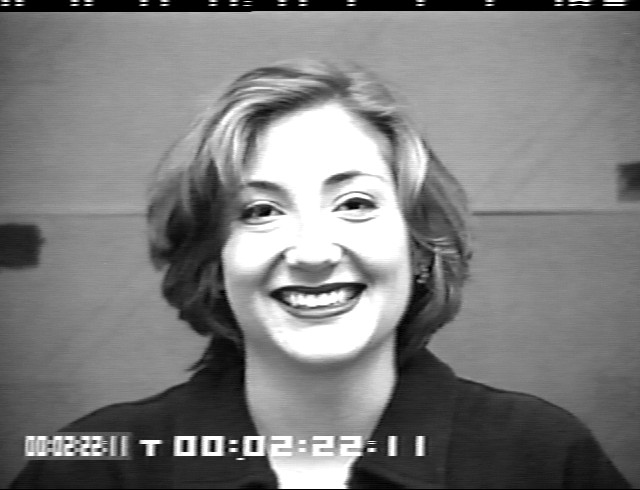
\includegraphics[width=\linewidth, height=0.3\paperheight, keepaspectratio]{ck_example.png}
	\caption{Primjer slike iz CK+ podatkovnog skupa}
	\label{pic:ck_example}
\end{figure}

\section{Ručno generirani podatkovni skup}
Slike CK+ podatkovnog skupa slikane su u istom okruženju (ista prostorija u kojoj se slikaju subjekti, ista kamera, slična svjetlina slike...). Nedostatak raznolikosti među slikama stvara potrebu za uvođenjem apstraktnijih slika ljudskih lica ne bi li model klasificirao emocije ljudskih lica koja nisu slična samo CK+ podatkovnom skupu. Zbog toga se uvodi podatkovni skup Google slika. Google omogućuje pretraživanje slika po zadanom upitu te dodatnim parametrima koji olakšavaju pronalaženje ljudskog lica koji predstavlja određenu emociju. Npr. pronalazak ljudskih lica koji iskazuju tužnu emociju mogao bi biti "sad human face" sa tipom Google slike "lice". Rezultati tog upita prikazani su na slici \ref{pic:google_search_sad}.

\begin{figure}[H]
	\centering
	
\includegraphics[width=\linewidth, height=0.3\paperheight, keepaspectratio]{2020-06-08-22-16-22.jpeg}
	\caption{Rezultati Google upita "sad human face"}
	\label{pic:google_search_sad}
\end{figure}

Rezultati ovog upita su slike veće raznolikosti (različit scenarij i drugačiji kut gledanja) što pridonosi apstrakciji emocije u ukupnom podatkovnom skupu. Dobivene slike ne odgovaraju uvijek nužno zadanom upitu zbog čega je potrebno dodatno provjeriti valjanost pojedine slike. Proces filtriranja objašnjen je u poglavlju \ref{google_npy_filter}


\section{Priprema podatkovnih skupova}\label{npy_preprocess}
\subsection{Priprema Cohn-Kanade podatkovnog skupa}
\subsubsection{Struktura podataka}

Dijelovi podatkovnog skupa značajni za treniranje dijele se na direktorij sekvence i emocije. Svaki subjekt (npr. S005) ima svoj direktoriji u kojem se nalaze pod direktoriji za emociju koju je subjekt odglumio (npr. 001, 002...) a u njemu se nalaze sekvence. Za 327 sekvenca postoji odgovarajuća emocija koja je definirana samo za krajnju sliku sekvence i njezina putanja je definirana jednako kao i za sekvencu.

\pagebreak

\begin{figure}[H]
\centering
\begin{Verbatim}[fontsize=\small]
├── emotions
│   ├── S005
│   │   └── 001
│   │       └── S005_001_00000011_emotion.txt
│   │       	└── "3.0000000e+00"
│   ├── S010
│   │   ├── 001
│   │   ├── 002
│   │   │   └── S010_002_00000014_emotion.txt
│   │   │   	└── "4.0000000e+00"
│   │   └── ...
│   └── ...
└── images
    ├── S005
    │   └── 001
    │       ├── S005_001_00000001.png
    │       ├── ...
    │       └── S005_001_00000011.png
    ├── S010
    │   ├── 001
    │   │   ├── S010_001_00000001.png
    │   │   ├── ...
    │   │   └── S010_001_00000013.png
    │   ├── 002
    │   │   ├── S010_002_00000001.png
    │   │   ├── ...
    │   │   └── S010_002_00000014.png
    │   └── ...
    └── ...

\end{Verbatim}
\caption{Struktura podataka CK+ podatkovnog skupa}
\label{cb:npy_tree}
\end{figure}

\subsubsection{Obrada podataka}
Jedina slika u sekvenci za koju je definirana emocija je zadnja slika, što znači da je potrebno je potrebno odrediti vektor emocije ostalih slika u sekvenci na temelju krajnje vrijednosti emocije. Emocija za pojedinu sliku definirana je kao red emocija. Svaki indeks reda predstavlja emociju kojih ima kojih ima 8. Indeks pojedine emocije definiran je na slici \ref{cb:emo_declare} a vrijednost na indeksu predstavlja intenzitet emocije

\begin{figure}[H]
\centering
\begin{Verbatim}[fontsize=\small]
emocije = {
    1: "neutral",
    2: "anger",
    3: "contempt",
    4: "disgust",
    5: "fear",
    6: "happy",
    7: "sadness",
    8: "surprise",
}
\end{Verbatim}
\caption{Deklaracija emocija}
\label{cb:emo_declare}
\end{figure}

\noindent
Znajući da je emocija za početnu sliku neutralna a za krajnju maksimalna sekvencijska emocija, emocije za ostale slike dodijeljene su linearno na način da se odredi intenzitet neutralne emocije \ref{eq:intensity_neutral} i sekvencijske emocije \ref{eq:intensity_seq} gdje je $n$ ukupan broj slika u sekvenci a $i$ slika kojoj se određuje vektor emocije.

\begin{equation}\label{eq:intensity_neutral}
	p_{n} = \dfrac{i-1}{n-1}	
\end{equation}
\begin{equation}\label{eq:intensity_seq}
\begin{split}
	p_{s} = 1 - p_{n}\\
	p_{s} + p_{n} = 1	
\end{split}
\end{equation}

\noindent
Primjer vektora emocije za sekvencu "disgust" koja sadrži 10 slika:

\begin{figure}[H]
\centering
\begin{tabular}{|c|c|} 
\hline
broj slike & vektor emocije \\
\hline
$i = 1$ & [1.0, 0.0, 0.0, 0.0, 0.0, 0.0, 0.0, 0.0] \\
... & ... \\
$i = 6$ & [0.4, 0.0, 0.0, 0.6, 0.0, 0.0, 0.0, 0.0] \\
... & ... \\
$i = n = 10$ & [0.0, 0.0, 0.0, 1.0, 0.0, 0.0, 0.0, 0.0] \\
$i$ & [$p_n$, 0.0, 0.0, $p_s$, 0.0, 0.0, 0.0, 0.0]  \\
\hline
\end{tabular}
\caption{Vektor emocije za pojedinu pojedinu sliku u sekvneci u CK podatkovnom skupu}
\label{pic:ck_emotion_rise}
\end{figure}



\subsubsection{Spremanje slike i vektora emocije u .npy podatak}\label{self:npy_save}
Za daljnje korištenje svaka slika i njezin vektor emocije će pretvorena u numpy red \cite{numpy_array} i spremljen kao .npy podatak. Prvi element numpy reda je slika a drugi je odgovarajući vektor emocije. Ovime je osigurano da izračun emocija za pojedinu sliku je izračunat samo jedanput što će smanjiti vrijeme potrebno za treniranje. Nakon provođenja transformacije podataka u .npy podatak ukupan broj slika i pripadajućih vektora emocija iznosi 5703. 



\begin{figure}[H]
	\centering
	\begin{subfigure}[b]{0.4\linewidth}
	  	\centering
		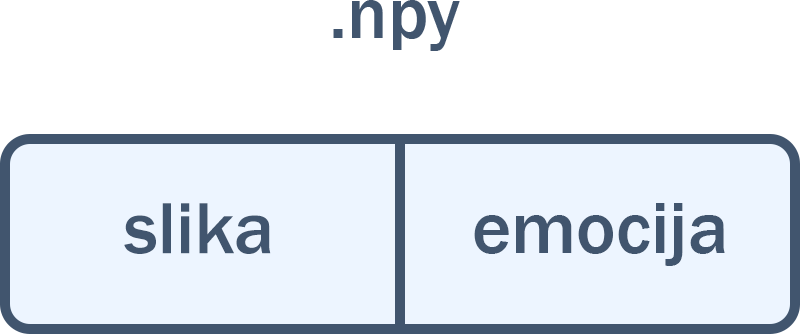
\includegraphics[width=\linewidth, keepaspectratio]{numpy_slika_emocija.png}
		\caption{Struktura .npy podatka}		
	\end{subfigure}
	\begin{subfigure}[b]{0.4\linewidth}
	  	\centering
		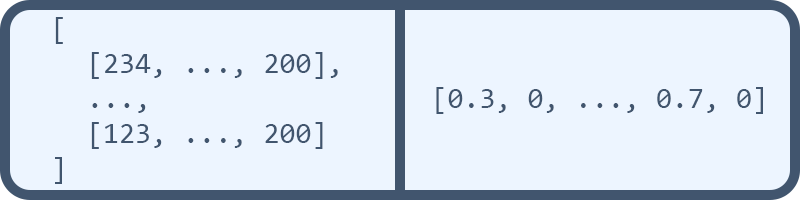
\includegraphics[width=\linewidth, keepaspectratio]{numpy_imgdata_emo.png}
		\caption{Sadržaj .npy podatka}
	\end{subfigure}	
	\caption{.npy podatak}	
	\label{fig:npy_array}
\end{figure}


\subsection{Priprema Google podatkovnog skupa}\label{priprema_google}
\subsubsection{Prikupljeni podaci}
Umjesto preuzimanja jedne po jedne slike korištena je google-images-download skripta \cite{google-images-download} koja preuzima sve moguće slike na temelju zadanog upita. Upiti korišteni za pronalaženje odgovarajućih emocija nalaze se na slici \ref{cb:google_queries} a svi su popraćeni dodatnim "Google search" parametrom koji pretražuje slike samo ljudskih lica. Svaka slika spremljena je u direktoriji čije je ime upit koji je bio korišten prilikom preuzimanje te slike. 

\begin{figure}[H]
	\centering
		\begin{Verbatim}[fontsize=\small]
		"sad human face"
		"neutral human face"
		"neutral expression"
		"angry human face"
		"angry expression"
		"contempt"
		"fear human face"
		"fear expression"
		"surprise human face"
		"surprise expression"
		"disgusted human face"
		"disgust expression"
		\end{Verbatim}
	\caption{Upiti za preuzimanje ljudskih lica sa Google-a}
	\label{cb:google_queries}
\end{figure}

\noindent
Nakon preuzimanja svih mogućih slika potrebno je ručno proći kroz svaki direktorij svakog upita i izbaciti slike koje ne zadovoljavaju sljedeće uvjete \label{google_npy_filter}

\begin{itemize}
	\item Na slici se nalazi samo jedno ljudsko lice
	\item Na slici se nalazi ljudsko lice čija emocija odgovara upitu pomoću kojeg je slika preuzeta
	\item Veličina slike je manja od 20MB
	\item Rezolucija slike je veća od 20px po duljini i visini
	\item Slika nije duplikat prethodno viđene slike
	\item Slika nije dio CK+ podatkovnog skupa
\end{itemize}
Uklanjanjem slika koje ne zadovoljavaju bilo koje od navedenih uvjeta dobiven ukupan broj slika povoljnih za treniranje iznosi 3160 a njihova ukupna veličina je 2,3GB.

\subsubsection{Struktura podataka}
Nakon filtriranja slika nepogodnih za treniranje potrebno je objediniti upite čiji su rezultati ljudska lica efektivno istih emocija. Primjer takva dva upita su "neutral human face" i "neutral expression". Nakon objedinjavanja rezultata upita i preimenovanja direktorija stvorena je struktura podataka dana na slici \ref{cb:google_file_structure}


\begin{figure}[H]
\centering
\begin{Verbatim}[fontsize=\small]
├── neutral
│   ├── 1.57053528-man-head-shot.png
│   ├── 2.Face_of_SpooSpa.png
│   ├── 3.main-1-low-res-4a61d.png
│   └── ...
├── anger
│   ├── 1.57053528-man-head-shot.png
│   └── ...
├── contempt
│   └── ...
├── disgust
│   └── ...
├── fear
│   └── ...
├── happy
│   └── ...
├── sadness
│   └── ...
└── surprise
    └── ...
\end{Verbatim}
\caption{Struktura podataka Google podatkovnog skupa}
\label{cb:google_file_structure}
\end{figure}

\subsubsection{Obrada podataka}
Obrada Google podatkovnog skupa bit će manje zahtjevna od CK+ podatkovnog skupa zbog toga što će se vektor emocije za pojedinu sliku odrediti samo na temelju upita korištenog za preuzimanje slike. Rezultat svakog vektora emocije bit će vektor dobiven metodom "One hot encoding". "One hot encoding" je metoda dodjele binarne vrijednosti za kategoriju u koju neki uzorak pripada ili ne pripada \cite{one_hot_encoding}. Ovom metodom uzorak (slika) može pripadati samo jednoj kategoriji (emocija). Slika koja pripada određenoj emociji za tu će emociju imati vrijednost 1 a za sve ostale 0. Na slici \ref{pic:google_emotion_emo_vector} prva kolumna označava ime direktorija u kojem se slike nalaze, druga kolumna predstavlja vektor emocije koje će slike u direktoriju poprimiti.

\begin{figure}[H]
\centering
\begin{tabular}{|c|c|} 
\hline
emocija (ime direktorija) & vektor emocije \\
\hline
neutral & [1,0,0,0,0,0,0,0] \\
anger	& [0,1,0,0,0,0,0,0] \\
contempt & [0,0,1,0,0,0,0,0] \\
disgust & [0,0,0,1,0,0,0,0]\\
fear  & [0,0,0,0,1,0,0,0]\\
happy & [0,0,0,0,0,1,0,0]\\
sadness & [0,0,0,0,0,0,1,0]\\
surprise & [0,0,0,0,0,0,0,1]\\
\hline
\end{tabular}
\caption{Vektor emocije za pojedinu emociju u Google podatkovnom skupu}
\label{pic:google_emotion_emo_vector}
\end{figure}

\subsubsection{Spremanje slike i vektora emocije u .npy podatak}
Nakon dodjele vektora emocije za pojedinu sliku potrebno je pretvoriti sliku i vektor emocije u .npy podatak. Kako se radi o slici i vektoru emocije, postupak pretvorbe slike i vektora emocije u pojedinačni .npy podatak jednak je kao i kod CK+ podatkovnog skupa definiranom u poglavlju \ref{self:npy_save}.


\subsection{Objedinjavanje podatkovnih skupova}
Nakon obrade CK+ i Google podatkovnog skupa svi .npy podaci bit će spremljeni u direktoriji "ck" ili "Google" ovisno o tome iz kojeg je podatkovnog skupa slika dobivena. Struktura svih .npy podataka prikazana je na slici \ref{pic:npy_structure}. Ovom strukturom moguće je definirati udio svakog podatkovnog skupa koji će biti korišten za treniranje modela. Poslije podjele u zasebne direktorije potrebno je odvojiti dio .npy podataka u test pod-direktoriji. U njemu će se nalaziti 20\% svih .npy podataka koji će modelu biti neviđeni prilikom treniranja. Tih 20\% .npy podataka koristit će se pri evaluaciji točnosti modela. Prikaz podjele podatkovnog skupa prikazan je na slici \ref{pic:dataset_split_percentages} Bitno je naglasiti da skup za evaluaciju ne smije ni u kojem trenutku biti izvor za treniranje mreže. Razlog toga je što model naučen na zadanom skupu slika će pri završetku treniranja biti u stanju sa vrlo visokom točnošću predvidjeti emociju slike koja je bila korištena prilikom treniranja. Evaluacija mora simulirati realnu situaciju u kojoj model nikad nije imao uvid u slike koje će biti korištene prilikom njegovog testiranja.

\begin{figure}[H]
	\centering
	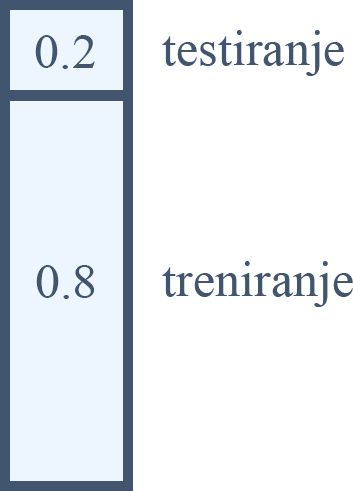
\includegraphics[width=\linewidth, height=0.3\paperheight, keepaspectratio]{splitset.png}
	\caption{Vizualni prikaz podijeljenog podatkovnog skupa}
	\label{pic:dataset_split_percentages}
\end{figure}

\begin{figure}[H]
\centering
\begin{Verbatim}[fontsize=\small]
numpy
├── ck
│   ├── test
│   │	├── test_slika_i_emocija_0001.npy
│   │	├── ...
│   │	└── test_slika_i_emocija_0570.npy
│   ├── slika_i_emocija_0001.npy
│   ├── ...
│   └── slika_i_emocija_5133.npy
└── google
    ├── test
    │	├── test_slika_i_emocija_0001.npy
	│	├── ...
	│	└── test_slika_i_emocija_0316.npy
    ├── slika_i_emocija_0001.npy
    ├── ...
    └── slika_i_emocija_2844.npy
    

\end{Verbatim}
\caption{Struktura .npy podataka}
\label{pic:npy_structure}
\end{figure}



\chapter{Treniranje}
Treniranje je proces u kojem model postupno mijenja svoje parametre ne bi li došao do idealnih parametara, čime bi model optimalno služio onome čemu je namijenjen. U slučaju klasifikacije za treniranje je potrebno imati skup podataka nad kojim će se provoditi treniranje i labele tih podataka koje govore klasu podataka. U slučaju klasifikacije emocija, skup podataka nad kojim se trenira su slike ljudskih lica dok je klasa emocija koja je prikazana na pojedinoj sliku. Kad treniranje započne, u model se pošalju podaci za koje model pokušava predvidjeti koje su klase ubačeni podaci. Nakon toga potrebno je usporediti predviđanja klasa koje je stvorio model sa pravim klasa. Pogrešku koju je model napravio prilikom predviđanja potrebno je javiti modelu ne bi li ispravio parametre. Mijenjanjem modela parametra model postaje sve bolji za predviđanje predviđanje rezultata na skupu za treniranje. Bitno je naglasiti da daljnjim treniranjem model ne postaje bolji za općeniti slučaj predviđanja. Treniranjem model se prilagođava podatkovnom skupu za treniranje. Podatkovni skup za treniranje je podskup svih podataka za koje je model namijenjen a to znači da skup za treniranje nije nužno najbolja mjera općenitog slučaja za podatke. 


Treniranje modela nakon određenog trenutka može pogoršati sposobnost modela da predviđa klase na općenitom slučaju. Uzrok toga je što treniranjem nakon određenog trenutka model ima veću točnost na skupu za treniranje ali točnost na općenitim, neviđenim slučajevima postaje sve manja. Zbog toga je potrebno pronaći optimalan trenutak u kojem treba prekinuti treniranje modela. Prekidanje treniranja modela nije moguće odrediti pomoću točnosti modela na skupu za treniranje jer ta točnost neprestano raste daljnjim treniranjem. Zbog toga je potrebno uvesti validacijski skup koji neće biti korišten prilikom treniranja. Validacijski skup o tom slučaju igra ulogu neviđenih podataka nad kojima se mjeri točnost. Prilikom treniranja točnost nad validacijskim skupom će rasti do optimalnog trenutka gdje je greška predviđanaj najmanja. U tom trenutku točnost nad validacijskim skupom će biti maksimalna a daljnjim treniranjem točnost će se smanjivati jer model postaje previše prilagođen skupu za treniranje \engl{overfitting}. Overfitting prikazan je na slici \ref{pic:overfitting}. Slika prikazuje overfitting zbog toga što prilikom treniranja greška validacija poslije optimalne točke greška nad validacijskim skupom postaje sve veća i veća.

\begin{figure}[H]
	\centering
	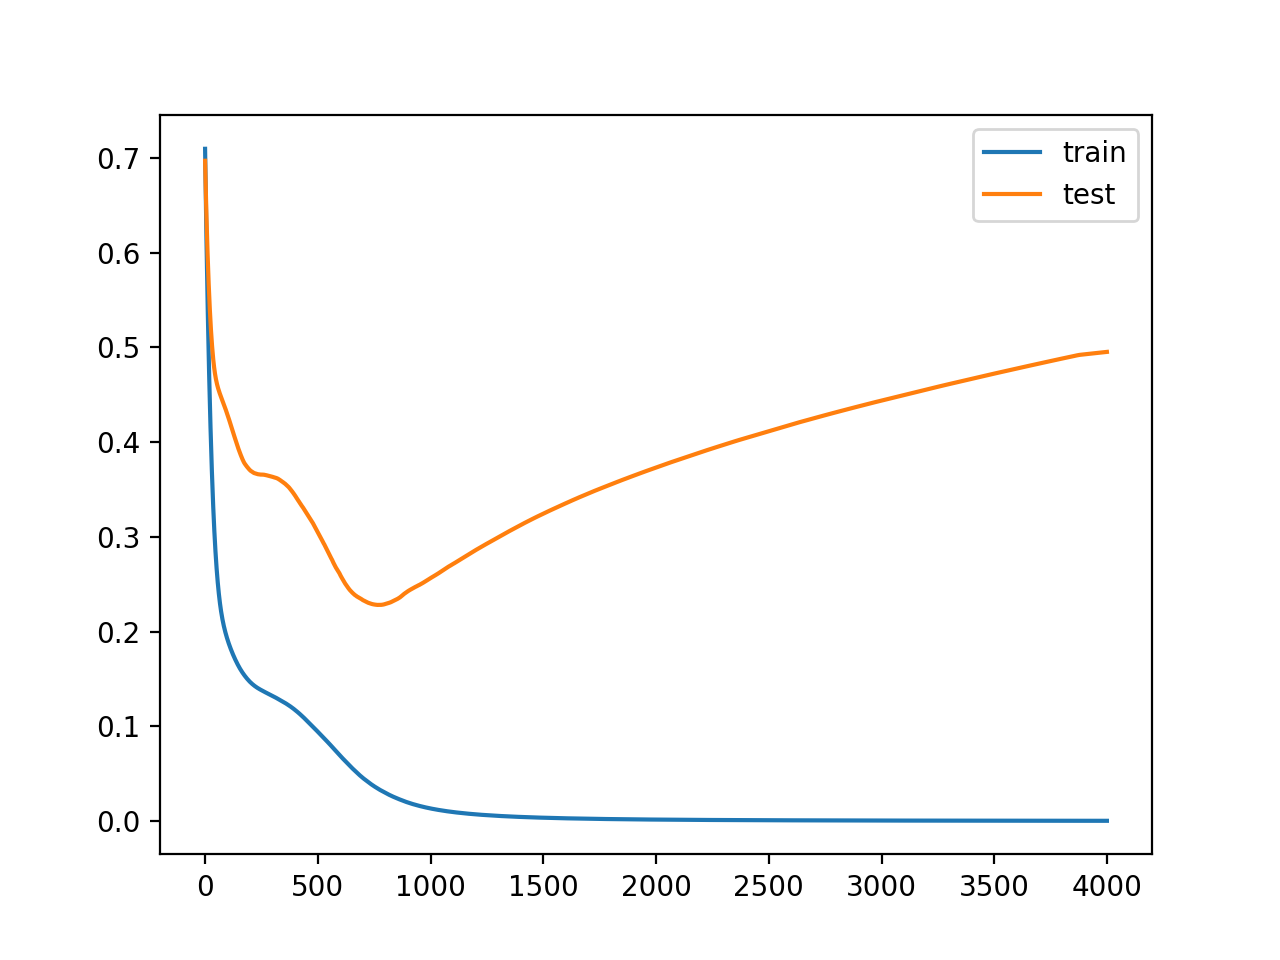
\includegraphics[width=\linewidth, height=0.3\paperheight, keepaspectratio]{overfitting.png}
	\caption{Primjer overfitting-a}
	\label{pic:overfitting}
\end{figure}


\section{Duboke neuronske mreže za analizu slika}
\subsection{Neuron}
Neuron je osnovni dio neuronske mreže. Svaki neuron na svoj ulaz prima vektor $x$ varijabli za koje neuron predviđa $\hat{y}$ izlaz. Skup $x$ vrijednosti pomnožen je sa vektorom $w$ koji predstavlja težine \engl{weights} i zbrojen sa vrijednošću $b$ koja predstavlja sklonost \engl{bias}. Težine neurona određuju povezanost između trenutnog i prethodnog neurona. Težištima neuroni utječu jedne na druge i određuju koliko su oni zavisni na prethodnom neuronu i za koje $x_i$ varijable. Parametri $w$ i $b$ su promjenjivi i mijenjaju se prilikom treniranja a $g$ je aktivacijska funkcija.


\begin{equation}\label{eq:neuron}
	\vect{z}=w_1x_1+w_2x_2+...+w_nx_n=\vect{w^{T}} \cdot \vect{x}
\end{equation}

\begin{equation}\label{eq:neuron_activation}
	\hat{y} = g(\vect{z})
\end{equation}

\subsection{Aktivacijska funckija}

Nakon zbrajanja unutar neurona, izlaz neurona potrebno je provesti kroz aktivacijsku funkciju koja određuje koliko je signal tog neurona bio zastupljen u ukupnom izlazu, tj. koliko je neuron "aktiviran". Aktivnost predstavlja vezu između dva neurona a vrijednost aktivnosti govori koliko će rezultat jednog neurona utjecati na rezultat drugog. Cilj koji se postiže tom funkcijom je izlaz neurona bude postane nelinearan čime cijela neuronska mreža postaje nelinearna. Kad bi neuronska mreža uistinu bila linearan model njezina bi bila jednako dobra kao i regresijski model. Uvođenjem aktivacijske funkcije neuronska mreža može aproksimirati funkcije više reda što znači da su granice klasifikacija te neuronske mreže podijeljene granicom odluke \engl{decision boundary} koja nije linearna. Primjer takvih funckija je sigmoid prikazan na slici \ref{fig:sigmoid} i rektifikacijska funckija ReLU \engl{Rectifier} prikazana na slici \ref{fig:relu}. Prilikom aktivacije neurona koristiti će se rektifikacijska funkcija zbog toga što je opće primjenjiva, daje dobre rezultate i računanje je znatno zbog jednostavnosti funkcije.


\begin{figure}[H]
	\centering
		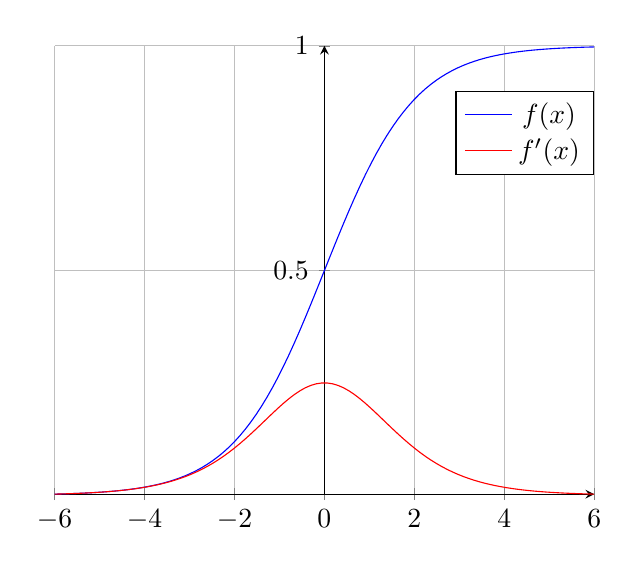
\begin{tikzpicture}[declare function={
			sigma(\x)=1/(1+exp(-\x));
			sigmader(\x)=sigma(\x)*(1-sigma(\x));
			},scale=1]
			
			\begin{axis}%
			[
			    grid=major,     
			    xmin=-6,
			    xmax=6,
			    axis x line=bottom,
			    ymax=1,
			    axis y line=middle,
			    ytick={0,.5,1},
			    samples=100,
			    domain=-6:6,
			    legend style={at={(1,0.9)}}     
			]
			    \addplot[blue,mark=none]   (x,{sigma(x)});
			    \addplot[red,mark=none]   (x,{sigmader(x)});
			    \legend{$f(x)$,$f'(x)$}
			\end{axis}
			\end{tikzpicture}
		\caption{Sigmoid}	
		\label{fig:sigmoid}	
\end{figure}		

\begin{figure}[H]
	\centering
		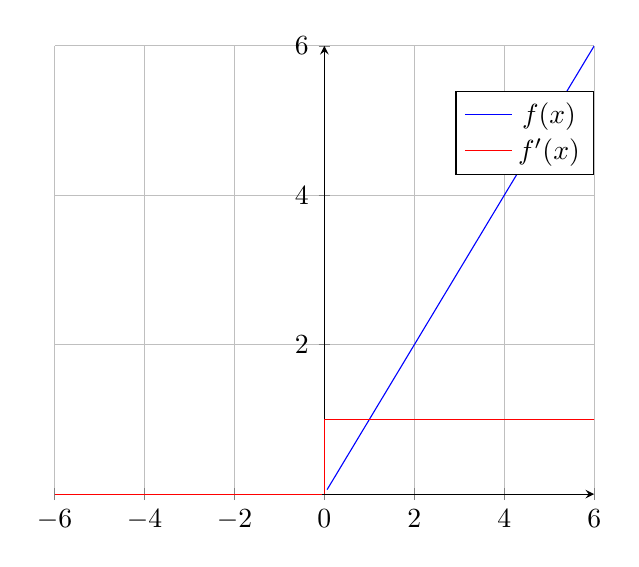
\begin{tikzpicture}[declare function={
			linear(\x)=\x;
			linearder(\x)=\x;
			},scale=1]
			
			\begin{axis}%
			[
			    grid=major,     
			    xmin=-6,
			    xmax=6,
			    axis x line=bottom,
			    ymax=6,
			    axis y line=middle,
			    samples=100,
			    domain=-6:6,
			    legend style={at={(1,0.9)}}     
			]	
			   \addplot[blue, restrict expr to domain={}{0:inf}]  (x,{linear(x)});
				\addplot[blue,  forget plot, restrict expr to domain={}{-inf:0}]  (x,0);
				\addplot[red, restrict expr to domain={}{-inf:0}]  (x,0);
				\addplot[red, const plot]  coordinates {(-inf,0) (0,0) (0,1) (100,1)};
			   \legend{$f(x)$,$f'(x)$}
			\end{axis}
			\end{tikzpicture}
		\caption{Linearna rektifikacijska funkcija \engl{ReLU}}
		\label{fig:relu}
\end{figure}

\subsection{Sloj neurona}

Sloj neurona sastoji se od skupa neurona. Matematički, sloj neurona sastoji se od prethodno aktiviranog izlaza $\vect{a_{l_{i-1}}}$ sloja $l_{i-1}$ i vektora $\vect{w_{l_{i}}}$ koji označava težišta za trenutni sloj $l_i$. U slučaju prvog sloja vrijedi $\vect{a} = \vect{x}$ jer prvi sloj ne ovisi ni o kojem prethodnom aktiviranom sloju. Račun izlaza sloja neurona računa se slično kao i kod pojedinog neurona. Za svaki sloj neurona $l_i$ izlaz $\vect{z}$ jednak je umnošku prethodne aktivacije $\vect{a_{l_{i-1}}}$ sa trenutnim težinama sloja neurona $\vect{w_{l_i}}$ zbrojen sa sklonošću $\vect{b_{l_i}}$. Izlaz neurona $\hat{y}$ dobiva se tako da se vektor $\vect{z}$ aktivira aktivacijskom funkcijom $g$, u ovom slučaju $g$ je funkcija ReLU prikazana na slici \ref{fig:relu}. Tako dobiven izlaz šalje se na sljedeći sloj neurona.

\begin{equation}\label{eq:neuron_layer}
	\vect{z_{l_i}} = \vect{w_{l_i}} \cdot \vect{a_{l_{i-1}}} + \vect{b_{l_i}}
\end{equation}

\begin{equation}\label{eq:neuron_layer_activation}
	\hat{y} = g(z)
\end{equation}

\subsection{Neuronska mreža}



Neuronska mreža sastoji se od više slojeva neurona koji su međusobno povezani. Slojevi su povezani tako što je svaki neuronski sloj razine $l_i$ povezan sa svakim neuronskim slojem razine $l_{i+1}$. Povezani su na način da se izlaz neuronskog sloja $l_i$ dovodi na ulaz neuronskog sloja $l_{i+1}$. Prije dovođenja na ulaz $l_{i+1}$ izlaz sloja $l_i$ proveden je kroz aktivacijsku funkciju $g$ čime je izlaz aktiviran. Ovaj algoritam prijenosa podataka s jednog sloja na drugi zove se \textit{feedforward} algoritam. Slojevi se dijele u tri različite grupe: ulazni, skriveni i izlazni sloj. Ulazni sloj je prvi sloj na koji se dovodi ulazni podataka, slika. Izlazni sloj je sloj koji na izlazu daje klasifikaciju ulazne slike, u ovom slučaju vektor predviđenih emocija. Skriveni slojevi su među-slojevi koji obrađuju podatke prethodnog izlaznog sloja neurona. U sredinom skrivenog područja obrađuje se najviše informacija 

\begin{figure}[H]
	\centering
	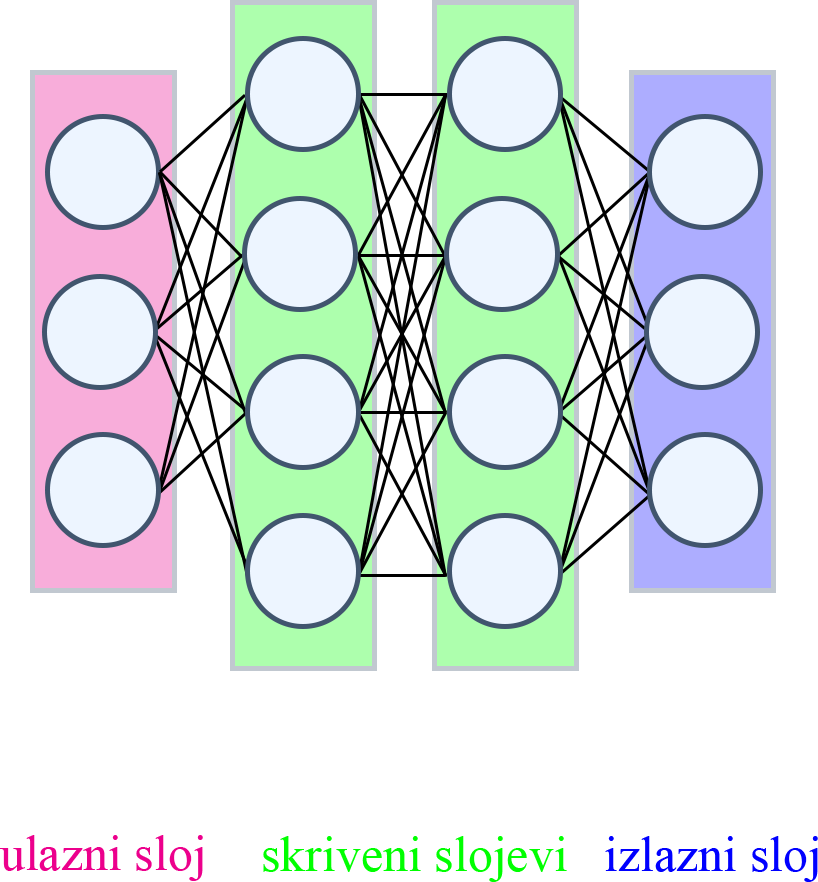
\includegraphics[width=\linewidth, height=0.3\paperheight, keepaspectratio]{neuron_layers.png}
	\caption{Različiti neuronski slojevi}
	\label{pic:ck_example}
\end{figure}

Što je neuronski sloj dublje razine to je apstrakcija podataka koju on računa veća. Izlaz skrivenog $l_i$ sloja poslat će se na ulaz sljedećeg skrivenog sloja $l_{i+1}$ a tim prijelazom apstrakcija podataka će biti uvećana. Uloga svakog neuronskog sloja je da obrađuje podatke na razini apstrakcije definiranje njegovom dubinom. Većim brojem slojeva neurona stvara se dublja neuronska mreža koja može računati na većoj razini apstrakcije. Interpretacija razine apstrakcije u slučaju slika svodi se na promatranje različitih djelova slike različite veličine. Iako se promatraju različiti dijelovi slike, međuzavisnost neuronskih slojeva omogućava neuronskoj mreži da zna koje je svojstvo slike proizašlo iz prethodnog svojstva slike. Primjer bi bio pronalaženje ruba usnice i ruba oka na slici.

\begin{figure}[H]
	\begin{subfigure}[b]{0.5\linewidth}
	  	\centering
		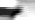
\includegraphics[width=\linewidth, height=0.3\paperheight, keepaspectratio]{usna_corner.png}
		\caption{Manji dio usnice, rub usnice}		
	\end{subfigure}
	\begin{subfigure}[b]{0.5\linewidth}
	  	\centering
		
\includegraphics[width=\linewidth, height=0.3\paperheight, keepaspectratio]{oko_corner.png}
		\caption{Manji dio oka, rub oka}
	\end{subfigure}	
	\caption{Slični rubovi djelova lica}	
	\label{fig:npy_array}
\end{figure}

Iako ta dva rubovi izgledom mogu biti slični bitna spoznaja za neuronsku mrežu je da jedan rub proizlazi iz slike usnice a drugi iz slike oka. Tako na primjer rub usnice usmjeren prema gore ukazuje na emociju sreće, dok to za rub oka ne mora biti slučaj. Ovakvo širenje konteksta bitno je za ispravno treniranje neuronske mreže.




\begin{figure}[H]
	\begin{subfigure}[b]{0.5\linewidth}
	  	\centering
		
\includegraphics[width=\linewidth, height=0.3\paperheight, keepaspectratio]{usna.png}
		\caption{Veći dio usnice}		
	\end{subfigure}
	\begin{subfigure}[b]{0.5\linewidth}
	  	\centering
		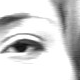
\includegraphics[width=\linewidth, height=0.3\paperheight, keepaspectratio]{oko.png}
		\caption{Veći dio oka}
	\end{subfigure}	
	\caption{Dijelovi lica}	
	\label{fig:npy_array}
\end{figure}




\subsection{Funkcija gubitka}\label{loss_function}
Funkcija gubitka \engl{loss function} je funkcija koja govori koliko je neuronska mreža daleko ili blizu rezultata koji se želi postići. Rezultat funkcije gubitka bit će pogreška koju je mreža napravila prilikom predviđanja vektora emocije određene slike. Taj rezultat bit će korišten za ispravljanje parametara neuronske mreže. Funkcija gubitka treba ukazati na kojim je predviđanjima neuronska mreža pogriješila i za koliko. Križni entropijski gubitak \engl{Cross Entropy Loss} je funkcija gubitka dana sa \ref{eq:cross_entropy} koja će biti korištena prilikom određivanja gubitka. Funkcija prima dva parametra, ispravna vrijednost označenu kao vektor $\vect{x}$ je i predviđenu vrijednost označenu kao vektor $\vect{y}$. U slučaju predviđanja emocija $\vect{x}$ je stvaran vektor emocije za pojedinu sliku dok je $\vect{y}$ previđen vektor emocije stvoren na izlazu neuronske mreže. Vektor $\vect{w}$ predstavlja težišta za pojedini element vektora $\vect{x}$ i $\vect{y}$. Elementi vektora $\vect{w}$ su $w_1, w_2, ..., w_n$ gdje svaki $w_i$ predstavlja koeficijent koji će biti pomnožen sa rezultatom gubitka. Razlog uvođenja težišta je neravnomjerna zastupljenost klasa u podatkovnom skupu za treniranje. Klase s manjim brojem uzoraka imat će veće težište prilikom računanja gubitka i samim time će biti "bitnije" prilikom treniranja. Kazna pogreške predviđanja za klasu emocije manjeg brojem uzoraka bit će veća nego u slučaju ne korištenja težišta. 

\begin{equation}\label{eq:cross_entropy}
	CrossEntropyWeighted\left(\vect{x}, \vect{y},\vect{w}\right) =
		-\sum_i w_i \left( x_i log\left(y_i \right)\right)
\end{equation}

\subsection{Treniranje neuronske mreže}\label{nn_train}

Neuronska mreža predstavlja nelinearnu funkciju koja se sastoji od $n$ varijabli a parametri su spomenuti parametri pojedinog neurona spomenuti na formuli \ref{eq:neuron}, težišta neurona $\vect{w}$2 i sklonost neurona $b$. Mijenjanje tih parametra parametra na način da se rezultat funkcije gubitka smanjuje naziva se treniranje. Cilj treniranja je minimizirati gubitak tako da se pronađe lokalni minimum u $n$ dimenzionalnom prostoru, gdje je broj $n$ broj varijabli u neuronskoj mreži. Metoda pronalaska minimuma zove se spuštanje gradijentom \engl{gradient descent}. Računanje spusta svodi se na izračun derivacije parametra neuronske mreže prema \ref{eq:graident_der} gdje je greška neuronskog sloja $E$, $a$ aktivacijski izlaz  i $w$ težina sloja.

\begin{equation}\label{eq:graident_der}
	\frac{\partial E}{\partial w} = \frac{\partial E}{\partial a} \cdot \frac{\partial a}{\partial w}
\end{equation}

Ovom jednadžbom dobiven je smjer negativnog gradijenta koji vodi ka minimumu n dimenzionalne plohe. Brzina kojom neuronska mreža konvergira prema minimumu označena sa $lr$ zove se stopa učenja \engl{learning rate}. Gradijent se računa prilikom svake iteracije treniranja, tj. nakon svakog dovođenja slike na ulaz mreže. Izračunati gradijent na sloju $l_i$ pomnožen sa stopom učenja $lr$ povratnom vezom se šalje na prethodni sloj $l_{i-1}$. Sloj $l_{i-1}$ koristiti će dobivenu vrijednost da ažurira svoja težišta sljedećim izračunom:

\begin{equation}\label{eq:gradient_backprop_layer}
	 w_{l_{i-1}} - lr \frac{\partial E_{l_i}}{\partial w_{l_i}} \rightarrow w_{l_{i-1}}
\end{equation}

Ovaj postupak naziva se backpropagration i primjenjuje se na sve slojeve neurona u neuronskoj mreži prilikom svake iteracije treniranja mreže.
 
\subsection{Rezidualna neuronska mreža}
\subsubsection{Motivacija}
Problem prilikom treniranja duboke neuronske mreže je mogućnost nestajućeg gradijenta \engl{vanishing gradient problem} pri ranim neuronskim slojevima mreže. Prilikom backprogragation algoritma sloj $l_i$ ažurirat će svoja težišta danom formulom \ref{eq:gradient_backprop_layer}. Bitno je naglasiti da vrijednost koja će ažurirati njegovo težište $lr \frac{\partial E_{l_n}}{\partial w_{l_n}}$ je gradijent izračunat od svih prethodnih slojeva $l_{i+1}, ..., l_n$. Ukoliko iznos gradijenta u više slučajeva bude manji od $1$ težište neurona će s vremenom početi konvergirati prema $0$. Što težište više konvergira prema $0$ to je teže ažurirati njegovu vrijednost.

Prilikom treniranja neuronske mreže ulaz $x$ koji prolazi kroz jedan neuronski sloj $l$ bit će izračunat formulom \ref{eq:neuron}. U nekim iteracijama treniranja poželjno je i izostaviti utjecaj nekog sloja $l$ jer njegov utjecaj ne mora nužno biti potreban za iteraciju treniranja. Drugim riječima ulaz $x$ prolazom kroz sloj $l$ treba ostati nepromijenjen, čime bi izlaz $y$ sloja $l$ bio jednak $x$. Funkcija čija je vrijednost za argument $x$ jednaka $x$ zove se funkcija identiteta dana na \ref{eq:identitiy_function}.

\begin{equation}\label{eq:identitiy_function}
f(x) = x
\end{equation}

U praksi neuronski sloj ne pronalazi funkcija identiteta s lakoćom jer metoda pronalaska funkcije identiteta zahtjeva računalnu snagu koja je aproksimacija funkcije identiteta.

Opisan postupak je posebno problematičan kad je neuronska mreža velike dubine. Suprotno intuiciji, dodavanjem većeg broja slojeva na neuronsku mrežu gubitak neće uvijek nužno biti smanjen. Nakon određenog broja slojeva dodavanjem novih slojeva gubitak prilikom treniranja postaje sve veći a time točnost predviđanja manja. Primjer ovog problema dan je na slici \ref{fig:deep_plain_error}.

\begin{figure}[H]
	\centering
	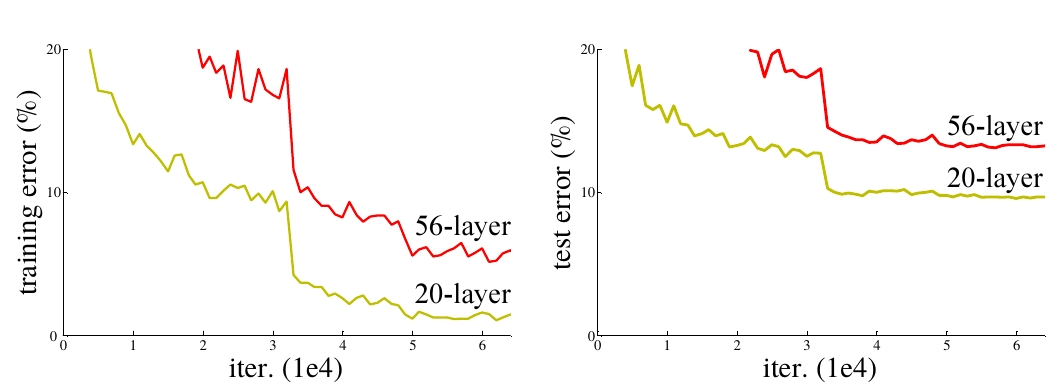
\includegraphics[width=\linewidth, height=0.3\paperheight, keepaspectratio]{deep_plain_error.jpeg}
	\caption{Pogreška prilikom treniranja obične duboke neuronske mreže ovisno o dubini mreže \cite{residual}}	
	\label{fig:deep_plain_error}
\end{figure}

\subsubsection{Rezidualni blok}

Rješenje problema spomenutog u motivaciji može se izbjeći korištenjem rezidualnog bloka. Taj prijedlog dan je prema  \cite{residual}. Umjesto aproksimiranja identifikacijske funkcije $f(x) = x$ uvodi se izraz pomoću kojeg se funkcija identiteta lako izračuna. 

\begin{equation}\label{eq:residual_identity}
f(x) \coloneqq h(x) + x
\end{equation}
\noindent
Sad je za neuronsku mrežu lako pronaći funkciju identiteta na način da se postavi $f(x) = 0$ čime se dobiva:

\begin{align*}
	& h(x) = f(x) + x \\
	& h(x) = x 
\end{align*}
\noindent
Ovime je osigurano da je originalan podatak $x$ moguće proslijediti sljedećem neuronskom sloju $l_{i+2}$ kroz neuronski sloj čak i ukoliko težišta $w$ sloja $l_i$ budu jednaka $0$. Čak i ako neuronski sloj ne djeluje na podatak $x$ on će ostati nepromijenjen čime je doprinos na buduće slojeve uvijek jednak ili bolji, što nije slučaj za obične duboke neuronske mreže. Ova činjenica omogućava dodavanje slojeva bez ikakvog gubitka točnosti. 

Implementacija rezidualnog bloka prikazan na \ref{fig:residual_block} ostvaruje se dodavanjem prečaca \engl{skip connection} između bloka $l_i$ i bloka $l_{i_2}$ koji služi da se podatak $\vect{x}$ koji se zbraja sa izlazom $f(x)$. 

\begin{figure}[H]
	\centering
	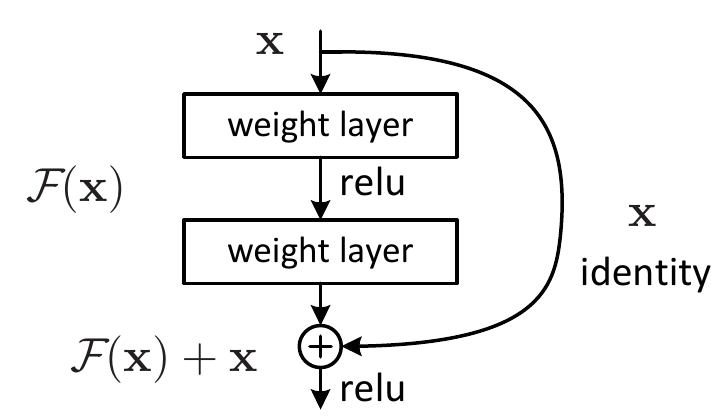
\includegraphics[width=\linewidth, height=0.3\paperheight,keepaspectratio]{resnet_block.jpeg}
	\caption{Pogreška prilikom treniranja obične duboke neuronske mreže ovisno o dubini mreže  \cite{residual}}
	\label{fig:residual_block}
\end{figure}


\noindent
Primjer izračuna izlaza korištenjem rezidualnog bloka za aktiviran ulaz $\vect{a_{l_i}}$, ReLU aktivacijsku funkciju $g$, težište $\vect{w_{l_i}}$ te prinos $\vect{b_{l_i}}$ gdje $l_i$ redni broj neuronskog sloja.
\begin{align*}
	& \vect{a}_{l_{i+2}}  = g(\vect{z}_{l_{i+2}} + \vect{a}_{l_i}) \\
	& \vect{a}_{l_{i+2}}  = g(\underbrace{\vect{w}_{l_{i+2}} \vect{a}_{l_{i+1}} + \vect{b}_{l_{i+2}}}_{0} + \vect{a}_{l_i}) \\
	& \vect{a}_{l_{i+2}}  = g(\vect{a}_{l_i}),\quad\text{$g$ je aktivacijska funckija ReLU}\\
	& \vect{a}_{l_{i+2}}  = \vect{a}_{l_i}
\end{align*}
\noindent
Ovime je pokazano da se po potrebi ulazni podatak lako može dobiti i na izlazu bez kompliciranih računskih operacija čime se izbjegava problema nestajućih gradijenta uz smanjenje korištenje računalne snage.

\subsubsection{Arhitektura mreže ResNet50}

Za stvaranje rezidualne neuronske mreže potrebno je ulančati više rezidualnih blokova. Konkretan rezidualan blok koji je korišten u ResNet50 arhitekturi prikazan je na slici \ref{fig:residual_block_50}. Cijela arhitektura ResNet50 mreže prikazana je na slici \ref{fig:resnet_arh} označena sa stupcem "50-layer". 

\begin{figure}[H]
	\centering
	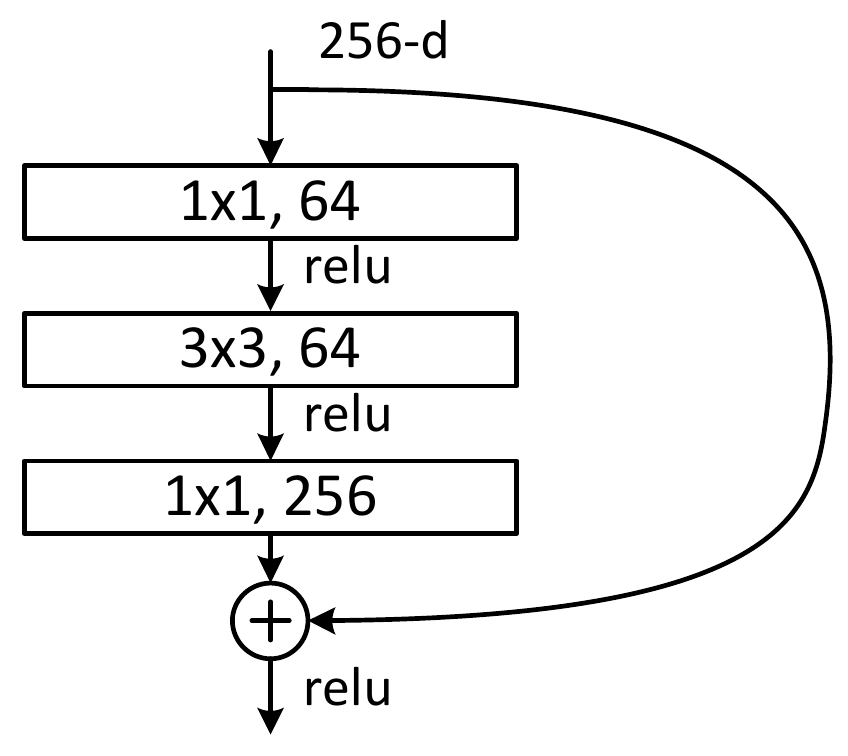
\includegraphics[width=\linewidth, height=0.3\paperheight,keepaspectratio]{resnet_50_block.jpeg}
	\caption{Rezidualni blok korišten u ResNet50 arhitekturi \cite{residual}}
	\label{fig:residual_block_50}
\end{figure}

\begin{figure}[H]
	\centering
	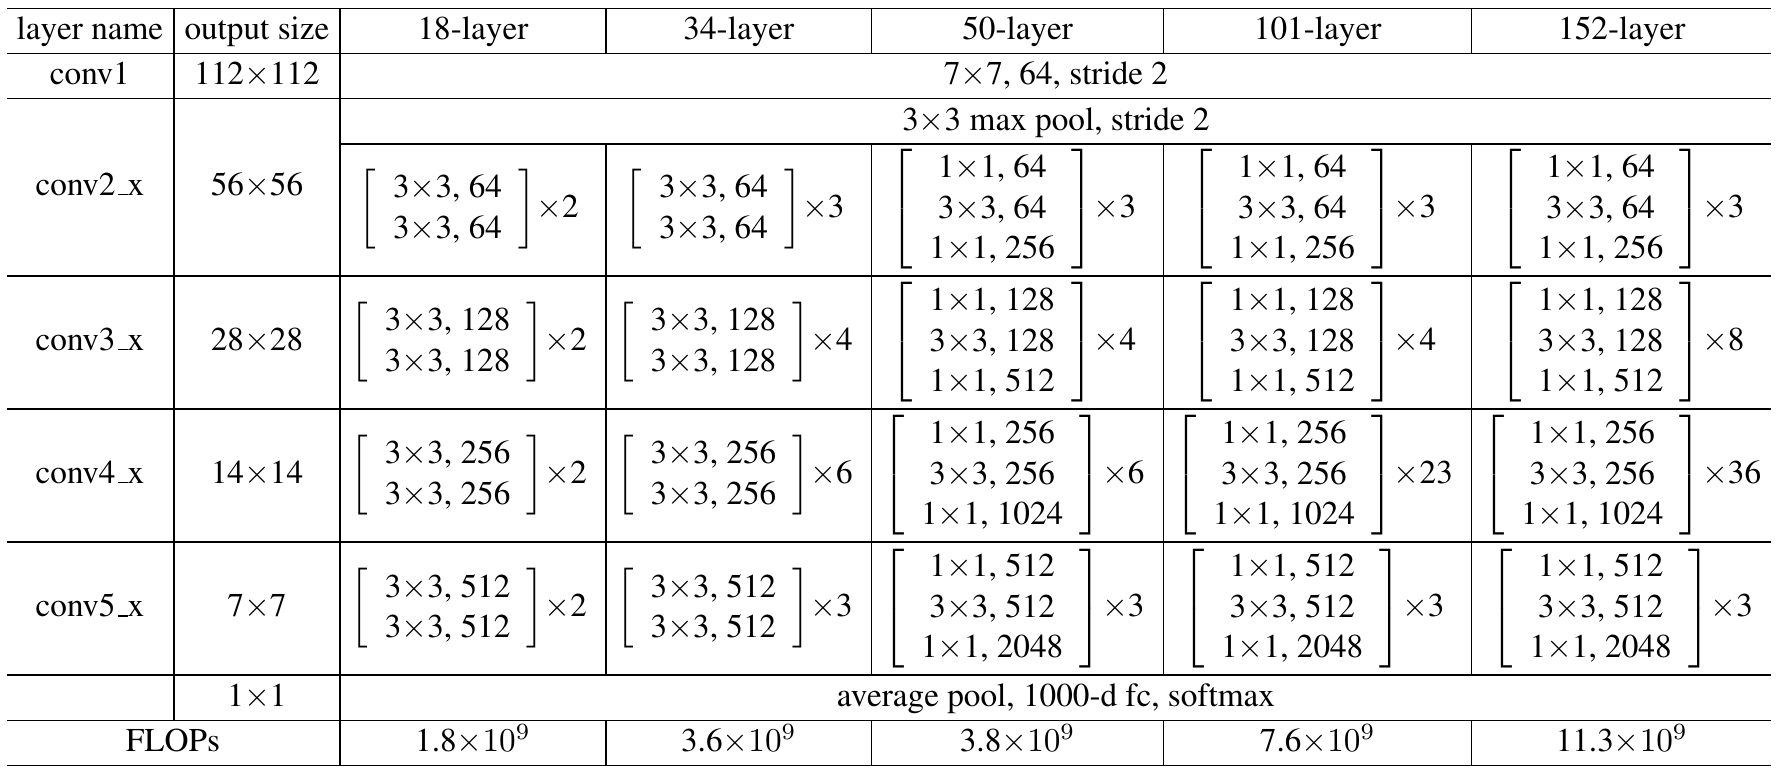
\includegraphics[width=\linewidth, height=0.3\paperheight,keepaspectratio]{resnet_arh.jpeg}
	\caption{ResNet50 arhitektura \cite{residual}}
	\label{fig:resnet_arh}
\end{figure}


Podaci dovedeni na ulaz ResNet50 mreže prolaze kroz nju sljedećim redoslijedom:
\begin{itemize}
	\item 1 sloj - Konvolucijski filter veličine $7\times7$ sa veličinom pomaka 2 koji slijedi konvolucijskim filterom veličine $3\times3$ uz maxpool metodu sa veličinom pomaka 2
	
	\item 9 slojeva
		\begin{itemize}
			\item Konvolucijski filter $1\times1$ ulaza veličine 64
			\item Konvolucijski filter $3\times3$ ulaza veličine 64
			\item Konvolucijski filter $1\times1$ ulaza veličine 256
			\item slojevi su ponovljeni 3 puta
		\end{itemize}
		
	\item 12 slojeva
		\begin{itemize}
			\item Konvolucijski filter $1\times1$ ulaza veličine 128
			\item Konvolucijski filter $3\times3$ ulaza veličine 128
			\item Konvolucijski filter $1\times1$ ulaza veličine 512
			\item slojevi su ponovljeni 4 puta
		\end{itemize}
		
	\item 18 slojeva
		\begin{itemize}
			\item Konvolucijski filter $1\times1$ ulaza veličine 256
			\item Konvolucijski filter $3\times3$ ulaza veličine 256
			\item Konvolucijski filter $1\times1$ ulaza veličine 1024
			\item slojevi su ponovljeni 6 puta
		\end{itemize}
		
	\item 9 slojeva
		\begin{itemize}
			\item Konvolucijski filter $1\times1$ ulaza veličine 512
			\item Konvolucijski filter $3\times3$ ulaza veličine 512
			\item Konvolucijski filter $1\times1$ ulaza veličine 2048
			\item slojevi su ponovljeni 3 puta
		\end{itemize}
		
		
\item 1 sloj - zadnji sloj je sloj prosječnog sažimanja čiji je izlaz veličine 1000 na koji djeluje funkcija "softmax" koja izlazne veličine pojedine klase pretvara u vjerojatnost prisutnosti klase. 
\end{itemize}

Ukupan broj navedenih slojeva je 50


\subsection{Prijenosno učenje}\label{transfered_learning}

Prijenosno učenje je tehnika u području strojnog gdje je naučenost modela za predviđanje jednog cilja prenesena na predviđanje drugog cilja. Potreba za ovom tehnikom javlja se iz nedovoljno velikog skupa podataka korištenog za treniranje. Zbog toga što podatkovni skup nije dovoljno velik, neuronska mreža neće biti dovoljno trenirana da predviđa emocija za neviđene slike. Unaprijed trenirana neuronska mreža ResNet50, koja je trenirana na ImageNet podatkovnom skupu \cite{imagenet}, omogućava mreži da od početka prepoznaje bitne značajke neviđene slike. Time je izbjegnuta potreba za treniranjem modela od početka jer su početni neuronski slojevi mreže već dobro naučeni za prepoznavanje bitnih značajki u slici, poput istaknutih objekta i uočljivijih oblika.

Zadnji slojevi unaprijed trenirane ResNet50 mreže mogu predviđati 1000 različitih značajki. Broj mogućih klasifikacijskih emocija je 8 zbog čega će biti potrebno dodati zadnji neuronski sloj na postojeću neuronsku mrežu tako da izlaz mreže bude dimenzije 8, a ne 1000 što odgovara broju različitih klasa korištenih u ImageNet podatkovnom skupu. Korištenjem većeg i apstraktnijeg podatkovnog skupa ova se tehnika može izostaviti.


\section{Implementacija treniranja u PyTorch-u}

\subsection{Uvod}

PyTorch okruženje je otvorenog koda \engl{open source} koja ubrzava proces implementacije strojnog učenja. Temeljne stvari strojnog učenja lakše je ostvariti u PyTorchu nego ručno pisati postupke nanovo. Iako PyTorch smanjuje kompleksnost koda i dalje je moguće po potrebi mijenjati detaljnije značajke i raditi promjene koje nisu nužno postojeće u trenutnom PyTorch okruženju pomoću nižeg Python okruženja. PyTorch će biti korišten prilikom učitavanja podataka, stvaranja podatkovnih skupova, inicijaliziranja hiperparametra, treniranja i testiranja.



\subsection{Oblikovanje podatkovnih skupova}
U poglavlju \ref{npy_preprocess} objašnjeno je stvaranje .npy podataka koji sadrže podatke slike i odgovarajućeg vektora emocije te slike. Sljedeći korak je iskoristiti te podatke za treniranje neuronske mreže koja će klasificirati emocije neviđenih slika ljudskih lica.

.npy podaci učitani su iz direktorija definiranog strukturom na slici \ref{pic:npy_structure}. Prilikom učitavanja .npy podataka koristiti će se parametri \lstinline"GOOGLE_TRAIN_SPLIT" i \lstinline"CK_TRAIN_SPLIT" pomoću kojih je moguće kontrolirati koji će udio slika iz pojedinog podatkovnog skupa biti zastupljen u skupu za treniranje.

\begin{figure}[H]
\centering
\begin{Verbatim}[fontsize=\small]
GOOGLE_TRAIN_SPLIT = 1
CK_TRAIN_SPLIT = 1
\end{Verbatim}
\caption{Udio .npy podataka pojedinog podatkovnog skupa}
\label{pic:split_dataset}
\end{figure}
\noindent
Sljedeći korak je stvaranje klase FERDataset \engl{Facial Recognition Dataset} koja implementira sučelja Dataset definiranog u PyTorchu. FERDataset sadrži dva argumenta: lokacija .npy podataka i funkcija za transformaciju slika. FERDataset sad ima pristup lokaciji .npy podataka i preko te lokacije će dohvaćati .npy podatke prilikom treniranja.
\begin{figure}[H]
\centering

\begin{Verbatim}[fontsize=\small]
class FERDataset(Dataset):
    def __init__(self, filepaths_numpy, transform_image=None):
        self.filepaths_numpy = filepaths_numpy
        self.transform_image = transform_image
\end{Verbatim}
\caption{Pojednostavljena inicijalizacija FERDataset}
\label{pic:init_dataset}

\end{figure}
\noindent
Prilikom dohvata .npy podataka preko funkcije \lstinline"__getitem__" .npy podatak je potrebno raspakirati u sliku lica i vektor emocije te slike. Ukoliko je zadana funkcija transformacije slike nju je potrebno primijeniti na sliku nakon raspakiravanja .npy podataka. Opis postupka transformacije slika nalazi se u poglavlju \ref{transform_image}. 


\begin{figure}[H]
\centering
\begin{Verbatim}[fontsize=\small]
def __getitem__(self, idx):
        name_npy = filepaths_npy(idx)
        image, emotion = load_npy(name_npy)
        image = transform(image)
        return image, emotion
\end{Verbatim}
\caption{Pojednostavljeni kod dohvata i raspakiravanja .npy podataka}
\label{pic:init_dataset}
\end{figure}

\subsubsection{Podjela podatkovnog skupa}
Inicijalizacijom klase koja implementira PyTorch sučelje Dataset, u ovom slučaju FERDataset, omogućeno je korištenje metoda koje lako mogu podijeliti podatkovni skup u skup za treniranje i evaluaciju. Podjela zasebnih .npy podataka već je odrađena u poglavlju \ref{npy_preprocess} a struktura direktorija podijeljenih .npy podataka dana je na slici \ref{pic:npy_structure} i \ref{pic:dataset_split_percentages}. Pomoću te dvije strukture, čija je putanja definirana sa varijablama \lstinline"FILEPATHS_NUMPY" i \lstinline"FILEPATHS_NUMPY", potrebno je stvoriti zasebni podatkovni skup za treniranje i evaluaciju. Na svaku od tih putanja prethodno djeluju navedene varijable \lstinline"GOOGLE_TRAIN_SPLIT" i \lstinline"CK_TRAIN_SPLIT" koje određuju udio zastupljenosti pojedinog podatkovnog skupa.

\begin{figure}[H]
\centering
\begin{Verbatim}[fontsize=\small]
train_dataset = FERDataset(filepaths_numpy=FILEPATHS_NUMPY,
                     transform_image=transform_image_train)
test_dataset = FERDataset(filepaths_numpy=FILEPATHS_NUMPY_TEST,
                          transform_image=transform_image_test)
\end{Verbatim}
\caption{Implementacija FERDataset klasa}
\label{pic:init_dataset}
\end{figure}

\subsubsection{Transformacija slike}\label{transform_image}

Prije nego što se podaci dobiveni iz \lstinline"train_dataseta" mogu koristiti za treniranje neuronske mreže potrebno ih je transformirati u pravilan oblik. Postupci transformiranja slike navedeni su ispravnim poretkom: 

\begin{itemize}
	\item{Promjena veličine} – iako je ovaj korak je već ostvaren u poglavlju \ref{npy_preprocess} promjena veličine slike bit će ponovno primijenjena iz sigurnosnih razloga. Sve slike lica su postavljene na fiksnu veličinu iznosa 224x224 piksela, \lstinline"IMG_SIZE = 224", zbog uzastopne mogućnosti dijeljenja broja sa 2, pogodna za ResNet50 arhitekturu u kojoj se dijelovi slike često prepolavljaju. Promjena veličine slike izvršava se s obzirom na centar slike.
	\item{Crno-bijelo} – slike lica su u crno-bijele slike iz razloga što boje na slici ne trebaju igrati ulogu u predviđanju emocija slike lica. Oblik, kontrast i rubovi na slici lica su dovoljno značajni za prepoznavanje ekspresije ljudskog lica. Crno-bijela transformacija ne mijenja trodimenzionalnu dimenziju boja slike već samo postavlja svaku od tri RGB boja na jednaku vrijednost.
	\item{Pretvorba u Tensor} – sliku ljudskog lica  potrebno je pretvoriti u tip podataka PyTorch Tensor \cite{pytorch_tensor} čime je PyTorch-u omogućeno da primjenjuje sve moguće ugrađene funkcije koje mogu djelovati na tip podataka PyTorch Tensor. Transformaciju koja slijedi inače nebi bilo moguće primijeniti.	 
	\item{Normalizacija} – korak prije slanja slike u neuronsku mrežu je normalizacija. Kako se koristi unaprijed trenirana neuronska mreža ResNet50, potrebno je provesti normalizaciju čiji parametri ovise o podatkovnom skupu koji su bili korišteni prilikom treniranja ResNet50 mreže. Ta normalizacija dana je od strane ImageNet-a \cite{normalize_imagenet} čiji je podatkovni skup korišten prilikom treniranja ResNet50 neuronske mreže.
\end{itemize}

Transformacije slika u PyTorch-u implementira se tako da se u \lstinline"transform.Compose" zada lista željenih transformacija. Redoslijed transformacija izvršavat će se poretkom elemenata u listi transformacija. Cjelokupnu transformaciju, kao argument pod imenom \lstinline"transform_image_train", u svom konstruktoru prima \lstinline"FERDataset", koji od sad ima pristup cjelokupnoj transformaciji. Kod i parametri transformacija dani su na slici \ref{pic:pytorch_transform}

\begin{figure}[H]
\centering

\begin{Verbatim}[fontsize=\small]
transform_image_train = transforms.Compose([
    transforms.Resize(IMG_SIZE),
    transforms.Grayscale(num_output_channels=3),
    transforms.ToTensor(),
    transforms.Normalize(mean=[0.485, 0.456, 0.406], std=[
        0.229, 0.224, 0.225])
])
\end{Verbatim}
\caption{Postupak transformacije slike}
\label{pic:pytorch_transform}
\end{figure}



\subsubsection{Augmentacija slike}


Augmentacija podataka \engl{data augmentation} je skup ne obaveznih transformacije koje povećavaju ukupnu apstraktnost podataka a samim time mogu stvoriti nepostojeće ali korisne podatke u skupu za treniranje. Ove transformacije simuliraju raznolik podatkovni skup na način da rade manje promjene na pojedinoj slici. Primjerice, nasumično povećavanje svjetline slike ili nasumična rotacija slike za kut \lstinline"-AUG_DEGREE". Na ovaj način neuronska mreža će naučiti klasificirati slike čak i ako su značajke poput svjetline slike i rotacije slične na cijelom podatkovnom skupu. To je upravo i slučaj u CK+ podatkovnom skupu. Sva su lica horizontalno poravnata čime a svjetlina slika je konzistentna.  Treniranje takvog podatkovnog skupa bez augmentacije, neuronska mreža će imati lošija predviđanja  emocije za slike lica gdje je lice blago zarotirano ili za znatno svjetlije ili tamnije neviđene slike. Uvođenjem augmentacije prilikom treniranja proširuje se primjena neuronske mreže koja kao rezultat može predviđati emocije za širu i apstraktniju domenu neviđenih slika. Augmentacija slike mora se obaviti prije normalizacije slike jer se augmentacija izvršava na slici kao takvoj a ne na PyTorch Tensor-u. Pojedina augmentacija primjenjivati će se nasumičnim intenzitetom za svaku sliku čime se osigurava da model ne bude pretreniran za specifičnu vrijednost augmentacije. 

 Augmentacije koje će biti korištene prilikom treniranja su:

\begin{itemize}
	\item{Nasumično horizontalno zrcaljenje} – često korištena augmentacija za koju će model bolje predviđati emocije za općenitije slike u kojima zrcaljenje slike ili kamere koja slika lice neće utjecati na rezultat predviđanja.
		
	\item{Promjena svjetline} - 
	
	\item{Rotacija slike} – nasumična rotacija između -15 i 15 stupnjeva
\end{itemize}



\noindent
Kod za potpunu transformaciju izgleda ovako:

\begin{figure}[H]
\centering
\begin{Verbatim}[fontsize=\small]
transform_image_train = transforms.Compose([
    transforms.Resize(IMG_SIZE),
    transforms.Grayscale(num_output_channels=3),
    transforms.RandomHorizontalFlip(),
    transforms.ColorJitter(brightness=1)
    transforms.RandomAffine(degrees=(-AUG_DEGREE, AUG_DEGREE)),
    transforms.ToTensor(),
    transforms.Normalize(mean=[0.485, 0.456, 0.406], std=[
        0.229, 0.224, 0.225])
])
\end{Verbatim}
\caption{Implementacija FERDataset klasa}
\label{pic:pytorch_transform_aug}
\end{figure}



\subsection{Hiperparametri}

\subsubsection{Funkcija gubitka}
Funkcija gubitka koja se koristi prilikom treniranja opisana je u poglavlju \ref{loss_function}\\
\begin{Verbatim}[fontsize=\small]
def CrossEntropyLossWeighted(pred, soft_targets, weights):        

    # logsoftmax umjesto logaritma jer
    # izlaz modela nije proveden kroz softmax
    logsoftmax = nn.LogSoftmax(dim=1)  
    
    plain_loss = - soft_targets * logsoftmax(pred)
    weighted_loss = weights * (plain_loss)
    result = torch.mean(torch.sum(weighted_loss, dim=1))
    return result
\end{Verbatim}
	
\subsubsection{Stopa učenja}
Definicija stope učenja napisana je u poglavlju \ref{nn_train} kao i područje na koje ona djeluje u formuli \ref{eq:gradient_backprop_layer}. Odabrana stopa učenja će biti postavljena na inicijalnu vrijednost 0.01 koja se dijeli sa 10 za svaku četvrtinu epohe, dakle vrijednosti su 0.01, 0.001, 0.0001, 0.00001. Razlog smanjivanja stope učenja prilikom treniranja je finija konvergencija prema minimumu. Ukoliko se ne koristi metoda smanjivanja stope učenja prilikom treniranja stopa učenja bit će postavljena na 0.0001.\\
\lstinline"LEARNING_RATE = 0.0001"

\subsubsection{Broj epoha}
Broj epoha \engl{epoch} je broj koji predstavlja koji će se puta treniranje provesti nad cijelim skupom za treniranje. Odabrana vrijednost je 100.\\
\lstinline"EPOCHS = 100"

\subsubsection{Veličina serije}
Veličina serije \engl{batch size} je veličina grupe slika koje se odjednom šalju neuronskoj mreži. Odabrana vrijednost iznosit će 16. To znači da će model u jednoj seriji predviđati emocije za 16 slika. Korištenjem serija funkcija gubitka kao rezultat vraća pogrešku za cijelu seriju.\\ \lstinline"BATCH_SIZE = 100"

\subsubsection{Slojevi ResNet50 mreže}
Spomenutu unaprijed treniranu mrežu ResNet50 potrebno je uvesti u projekt. Srećom, PyTorch već ima ugrađenu unaprijed treniranu ResNet50 mrežu treniranu nad bogatim podatkovnim skupom ImageNet \cite{imagenet}. Prilikom treniranja mreže koristi se metoda prijenosnog učenja, više u poglavlju \ref{transfered_learning}, gdje su svi slojevi mreže već unaprijed trenirani. Konvencija prilikom prijenosnog učenja je zamrznuti slojeve odgovorne za prepoznavanje početnih i temeljnih djelova slika, poput većih objekata, rubova i geometrijskih oblika. Težine preostalih slojeva bit će ažurirane prilikom treniranja za specifičan problem klasifikacije, u ovom slučaju klasifikacija emocije. Kako je ResNet50 trenirana na 1000 raznovrsnih klasa ima vrlo dobru mogućnost prepoznavanja raznolikih objekta na slici. U ovom slučaju slike lica su i dalje raznolika no postoje značajke na slikama lica koje su uvijek zajedničke (prisutnost različitih djelova lica). Zbog toga će zamrznuti slojevi biti svi osim zadnja tri sloja. Kad bi problem klasifikacije bio sličan podatkovnom skupu ImageNet zamrzavanje bi se provelo nad svim slojevima ResNet50 mreže.
\begin{Verbatim}[fontsize=\small]
resnet50 = models.resnet50(pretrained=True)

# zamrzavanje svih slojeva osim zadnja 3
for model_block in list(resnet50.children())[:-3]:
        for param in model_block.parameters():
            param.requires_grad = False
\end{Verbatim}


\subsubsection{Optimizator}
Optimizator koji će utjecati na mijenjanje težišta neurona prilikom backpropagation algoritma je optimizator Adam \cite{adam}. Za pronalaženje optimalnog rješenja, Adam koristi stohastički gradijentni spust uz moment djeluje na brzinu konvergencije prilikom iteracije. Moment djeluje na svaku varijablu koja se trenira.\\
\lstinline"optimizer = optim.Adam(resnet50.parameters(), lr=LEARNING_RATE)"



\subsection{Treniranje}

Inicijalizacijom svih potrebnih hiperparametara mreža je spremna za treniranje. Jedna iteracija treniranja izvršava se nad cijelim podatkovnim skupom za treniranje. Broj takvih iteracija bit će izvršen \lstinline"EPOCHS" puta. Prije početka treniranja potrebno je model prebaciti u stanje \lstinline"train" čime je označeno da će model mijenjati svoja težišta prilikom iteracija. Prilikom iteracija jedne epohe događa sljedeće:

\lstinline"train_loader" dohvaća jednu seriju podataka \lstinline"batch". Iz serije se izvlače podaci \lstinline"face" i \lstinline"emotions". To su lista slika i emocija a obje liste sadržavaju \lstinline"BATCH_SIZE" tj. 16 unikatnih slika lica i odgovarajućih emocija koje više neće biti dohvaćene prilikom trenutne epohe. 16 slika lica šalju se u model koji kao izlaz vraća 16 predviđenih emocija na temelju slika koje je upravo vidio. Funkcija gubitka \engl{loss function} uspoređuje predviđanja modela sa istinitim vektorom emocija \lstinline"loss_func(...)" tako da računa gubitak koji je model proizveo svojim predviđanjem, točnije, koliko je model pogriješio prilikom predviđanja emocije za slike trenutne serije. Funkcija gubitka nakon toga računa derivacije gubitka za svaki parametar \lstinline"loss.backwards()" a optimizator Adam koristi izračunate derivacije i stopu učenja da ažurira težišta modela \lstinline"optimizer.step()". Prije izračuna derivacija optimizator izbriše prethodno izračunate derivacije prošle serije pozivom \lstinline"optimizer.zero_grad()".
	
\begin{figure}[H]
\centering
\begin{Verbatim}[fontsize=\small]
for epoch in range(EPOCHS):

        train_loss = 0.0
        batch_loss = 0
        val_loss = 0

        model.train()
        for batch in train_loader:
            face, emotions = batch
            optimizer.zero_grad()
            outputs = model(face) # not softmaxed
            emotions = emotions
            loss = loss_func(pred=outputs.float(),
                             soft_targets=emotions.float(),
                             weights=WEIGHTS)
            loss.backward()
            optimizer.step()
            # emotion size is same as batch size
            train_loss += float(loss) * int(emotions.size(0)) 

        train_loss = train_loss / train_size
        train_losses.append(train_loss)
\end{Verbatim}
\caption{Pojednostavljen kod treniranja modela}
\label{pic:pytorch_transform_aug}
\end{figure}

Treniranje modela prestaje nakon \lstinline"EPOCHS" epoha a sprema se svaki model koji je bolji od najboljeg prethodnog. Ovime do tad najbolji model biti spremljen čak i ukoliko treniranje prestane prerano. Najbolji model mjeren je po kriteriju točnosti nad testnim podatkovnim skupom koji će biti objašnjen u sljedećem poglavlju.
\begin{Verbatim}[fontsize=\small]
if(epoch_acc > best_acc):
	best_acc = epoch_acc
	best_model = copy.deepcopy(resnet50.state_dict())
	torch.save(best_model, filename)
\end{Verbatim}

\begin{figure}[H]
	\centering
	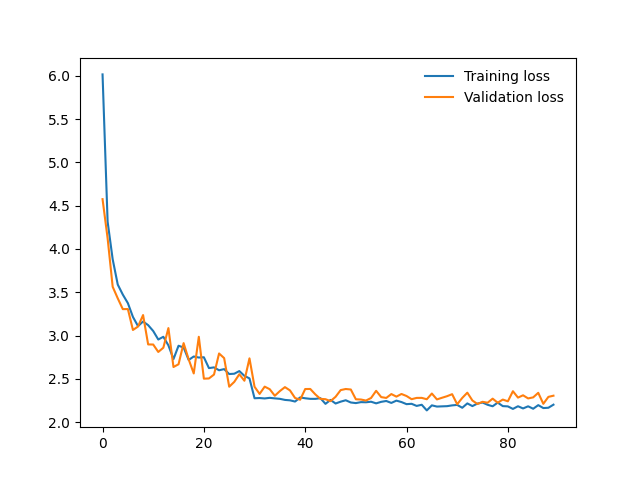
\includegraphics[width=\linewidth, height=0.3\paperheight, keepaspectratio]{val_ck.png}
	\caption{Greška prilikom treniranja nad podatkovnim skupom Google i CK+. Vertikalna os predstavlja iznos greške, horizontalna os broj epohe}
	\label{loss_ck}
\end{figure}

\chapter{Rezultati}

Nakon treniranja potrebno je detaljnije provjeriti rezultate, tj. predviđanja koje trenirani model daje za testni podatkovni skup nad kojim se nije treniralo. Testni podatkovni skup čini spomenutih 20\% ukupnog podatkovnog skupa. Prilikom odabira modela uzet će se model čija je točnost bila najveća nad testnim podatkovnim skupom jer je to model koji je sigurno najtočniji. Model koji ima najmanji gubitak nije nužno najbolji zbog oscilacija koje se javljaju prilikom treniranja sa veličinom serije veće od 1. 

Kao i kod treniranja, varijable \lstinline"GOOGLE_TRAIN_SPLIT" i \lstinline"CK_TRAIN_SPLIT" određuju udio pojedinog podatkovnog skupa prilikom treniranja. Ovime je omogućeno pojedinačno testiranja na svakom podatkovnom skupu kao i testiranje na oba podatkovna skupa.

Točnost predviđanja će se provesti će se tako da se predviđa prvih n dominantnih emocija:
za, n = 1 u slučaju Google podatkovnog skupa a n = 2 u slučaju CK+ podatkovnog skupa. Razlog toga je što istinite vrijednosti emocija za CK+ podatkovni skup predstavljaju dvije emocije čiji zbroj daje 1 dok je za Google podatkovni skup emocija određena jednom emocijom vrijednosti 1.

Svaka emocija bit će kodirana sljedećim riječima:
\begin{itemize}
\item{neutralno $\rightarrow$ neut}
\item{bijes $\rightarrow$ angr}
\item{prezir $\rightarrow$ cont}
\item{gađenje $\rightarrow$ disg}
\item{strah $\rightarrow$ fear}
\item{sreća $\rightarrow$ hppy}
\item{tuga $\rightarrow$ sadd}
\item{iznenađenje $\rightarrow$ surp}


\end{itemize}
\subsection{Rezultati za CK+ podatkovni skup}

Mreža nije imala većih problema prilikom predviđanja emocije jer je CK+ bio dominantan skup prilikom treniranja. Iako su slike za testiranje bile neviđene prilikom treniranja, one su slične strukturom, slikane istom kamerom a svi subjekti se nalaze u uglađenim kontroliranim uvjetima i gledaju direktno u kameru. Sve navedene značajke omogućavaju modelu da lakše predviđa emocija za slike s tim značajkama. 

\begin{figure}[H]
\centering
		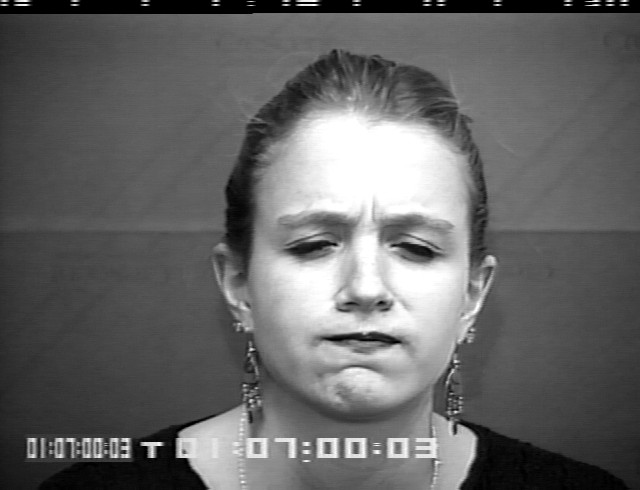
\includegraphics[width=0.3\linewidth, keepaspectratio]{S055_004_00000015.png}
		\begin{tabular}
					{|c|c|}\hline
					Emocije & [neut, angr, cont, disg, fear, hppy, sadd, surp]\\
					Istinita emocija & [0.49, 0.51, 0.00, 0.00, 0.00, 0.00, 0.00, 0.00]\\
					Predviđena emocija	& [0.21, 0.79, 0.00, 0.00, 0.00, 0.00, 0.00, 0.00]\\
					Pogođena dominantna emocija & 1\\
					Preciznost [0-1] & 0.72\\
					\hline
		\end{tabular}
\end{figure}

Predviđena emocija na slici iznad malo je izraženija nego što je istinita emocija iako je to i na slici čak i slučaj. Emocija nije u potpunosti izražena niti se sa sa sigurnošću može reći koliko je emocija neutralna. Intuicija mreže je da predvidi emociju kao intenzivnijom ako su promjene na licu znatnije.

\begin{figure}[H]
\centering
		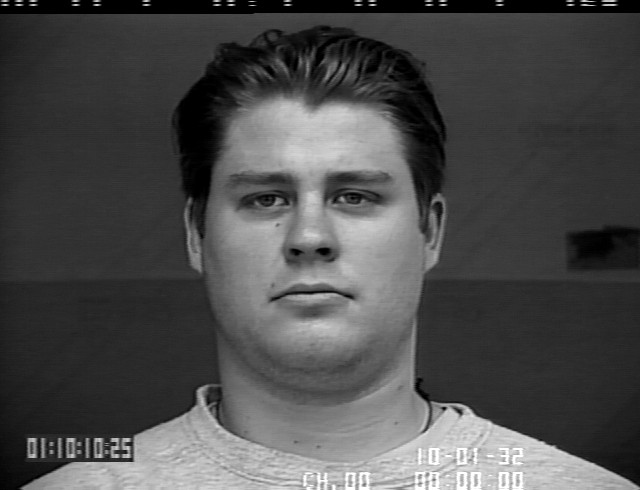
\includegraphics[width=0.3\linewidth, keepaspectratio]{S132_002_00000006.png}
		\begin{tabular}
					{|c|c|}\hline
					Emocije & [neut, angr, cont, disg, fear, hppy, sadd, surp]\\
					Istinita emocija & [0.70, 0.00, 0.00, 0.00, 0.00, 0.00, 0.29, 0.00]\\
					Predviđena emocija	& [0.93, 0.00, 0.00, 0.00, 0.00, 0.00, 0.07, 0.00]\\
					Pogođena dominantna emocija & 1\\
					Preciznost [0-1] & 0.75\\
					\hline
		\end{tabular}
\end{figure}
Previđena emocija je opravdano neutralnija nego što istinita emocija pokazuje. Pogreška ovakvog tipa nije značajna.

\begin{figure}[H]
\centering
		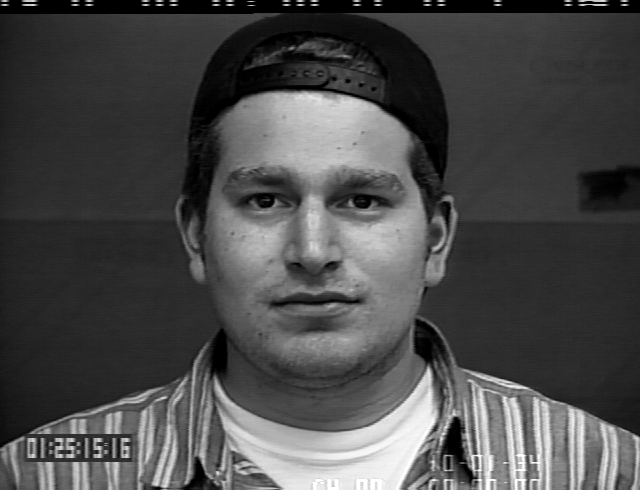
\includegraphics[width=0.3\linewidth, keepaspectratio]{S134_008_00000002.png}
		\begin{tabular}
					{|c|c|}\hline
					Emocije & [neut, angr, cont, disg, fear, hppy, sadd, surp]\\
					Istinita emocija & [0.90, 0.00, 0.00, 0.08, 0.02, 0.00, 0.00, 0.00] \\
					Predviđena emocija	& [0.55, 0.00, 0.00, 0.45, 0.00, 0.00, 0.00, 0.00] \\
					Pogođena dominantna emocija & 1\\
					Preciznost [0-1] & 0.62\\
					\hline
		\end{tabular}
	\caption{}
	\label{aa}
\end{figure}

Emocija gađenja po prirodi nije intenzivna s obzirom na ostale emocije zbog čega ju neuronska mreža teže prepoznaje. Promjene na licu su blage zbog čega je dodijeljena vrlo neutralna emocija.

\begin{figure}[H]
\centering
		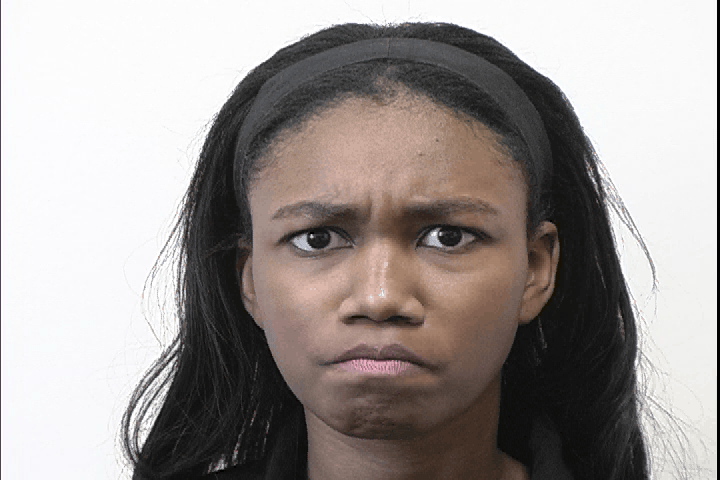
\includegraphics[width=0.3\linewidth, keepaspectratio]{S501_001_00000065.png}
		\begin{tabular}
					{|c|c|}\hline
					Emocije & [neut, angr, cont, disg, fear, hppy, sadd, surp]\\
					Istinita emocija & [0.03, 0.97, 0.00, 0.00, 0.00, 0.00, 0.00, 0.00] \\
					Predviđena emocija	& [0.04, 0.96, 0.00, 0.00, 0.00, 0.00, 0.00, 0.00] \\								Pogođena dominantna emocija & 1\\
					Preciznost [0-1] & 0.98\\
					\hline
		\end{tabular}
\end{figure}

Struktura lica ukazuje na ljutito lice za koju je mreža uspjela odrediti klasifikaciju i intenzitet. 

Model je za CK+ podatkovni točno predvidio emocije u 83\% slučajeva. Glavni razlog zbog kojeg točnost nije još i veća je što model teže prepoznaje granične slučajeve emocija kad emocija prelazi iz neutralne u jednu od preostalih sedam. Model ima sklonost da predvidi neutralnu emociju kao dominantnu iako to nije slučaj. Način odjeljivanja emocije linearnim rastom od neutralne do jedne od preostalih sedam nije nužno najbolja metoda određivanja pravih emocija. Aktivacija svake emocije može se za svakog subjekta dogoditi u drugačijem vremenskom trenutku. Najveći problem imala je emocija tuge a neutralna emocija bila je najviše puta pogođena. 






\begin{figure}[H]
\centering
		\begin{tabular}
					{|c|c|}\hline
					Emocije & [neut, angr, cont, disg, fear, hppy, sadd, surp]\\
					Preciznost emocija& [0.98, 0.76, 0.72, 0.78, 0.73, 0.81, 0.61, 0.73] \\
					Ukupna točnost predviđanja & 83\%\\
					\hline
		\end{tabular}
		\caption{Rezultati testiranja CK+ podatkovnog skupa}
\end{figure}


\subsection{Rezultati za Google podatkovni skup}


Google podatkovni skup je mnogo apstraktniji što ste tiče sadržaja slika s obzirom na CK+ podatkovni skup. Samim time je teže i trenirani model za predviđanje emocija takvih slika. Dodatan utjecaj na koji treba skrenuti pozornost su automatski preuzete slike na temelju ključnih riječi sa Googla. Iako su slike ručno filtrirane, i dalje postoje slike koje nužno ne odgovaraju ključnoj riječi pomoću koje su preuzete.




\begin{figure}[H]
\centering
		
\includegraphics[width=0.3\linewidth, keepaspectratio]{139a57640598.png}
		\begin{tabular}
					{|c|c|}\hline
					Emocije & [neut, angr, cont, disg, fear, hppy, sadd, surp]\\
					Istinita emocija & [0.00, 0.00, 0.00, 1.00, 0.00, 0.00, 0.00, 0.00]\\
					Predviđena emocija	& [0.00, 0.00, 0.00, 0.39, 0.57, 0.00, 0.01, 0.00]\\								Pogođena dominantna emocija & 0\\
					Preciznost [0-1] & 0.40\\
					\hline
		\end{tabular}
\end{figure}


Dio lica je prekriven zbog čega je odmah teže za model predvidjeti emociju. Iako začepljen nos ukazuje na emociju gađenja takva gesta nije bila često prisutna prilikom treniranja. Samim time model nije naučen da začepljen nos povezuje sa gađenjem. Strah koji dominantno predviđa temelji na spuštenim obrvama i blago zaokrenutim usnicama.

\begin{figure}[H]
\centering
		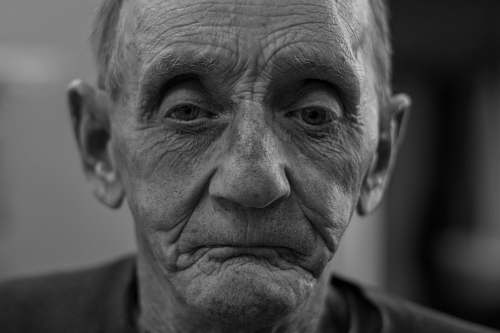
\includegraphics[width=0.3\linewidth, keepaspectratio]{84apeople-man-making-sad-face-person-person-image.png}
		\begin{tabular}
					{|c|c|}\hline
					Emocije & [neut, angr, cont, disg, fear, hppy, sadd, surp]\\
					Istinita emocija & [0.00, 0.00, 0.00, 0.00, 0.00, 0.00, 1.00, 0.00]\\
					Predviđena emocija	& [0.00, 0.00, 0.06, 0.00, 0.00, 0.00, 0.94, 0.00]\\
					Pogođena dominantna emocija & 1\\
					Preciznost [0-1] & 0.94\\
					\hline
		\end{tabular}
\end{figure}

Na subjektu su crte lice blago spuštene prema dolje čime subjekt sam po sebi iskazuje emociju tuge na temelju same slike. Uz tužan pogled i usnice nakrivljene prema dolje model nije imao problema predvidjeti dominantnu emociju.

\begin{figure}[H]
\centering
		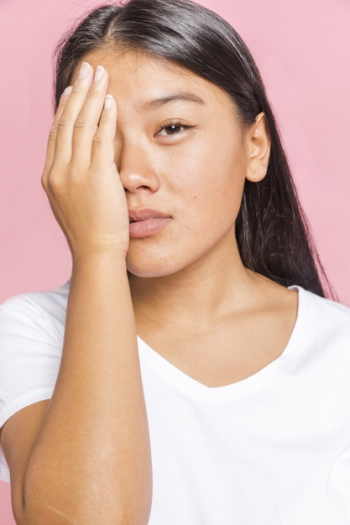
\includegraphics[width=0.3\linewidth, keepaspectratio]{210aae2259c476fa427d9c75.png}
		\begin{tabular}
					{|c|c|}\hline
					Emocije & [neut, angr, cont, disg, fear, hppy, sadd, surp]\\
					Istinita emocija & [0.00, 0.00, 0.00, 1.00, 0.00, 0.00, 0.00, 0.00]\\
					Predviđena emocija	& [0.40, 0.00, 0.00, 0.00, 0.00, 0.00, 0.58, 0.00]\\
					Pogođena dominantna emocija & 0\\
					Preciznost [0-1] & 0\\
					\hline
		\end{tabular}
\end{figure}

Model je u potpunosti pogriješio previđenu emociju, s razlogom. Na temelju istinite emocije lice bi trebalo predstavljati potpuno gađenje iako to nije slučaj. Iako je model pogriješio, njegov rezultat ima smisla. Spuštene oči gađenja zamijenio je sa tugom a neutralna emocija proizlazi iz blage emocije. Također, prekriven dio lica sigurno modelu otežava predviđanje emocije.

\begin{figure}[H]
\centering
		
\includegraphics[width=0.3\linewidth, keepaspectratio]{57aangry-main.png}
		\begin{tabular}
					{|c|c|}\hline
					Emocije & [neut, angr, cont, disg, fear, hppy, sadd, surp]\\
					Istinita emocija & [0.00, 1.00, 0.00, 0.00, 0.00, 0.00, 0.00, 0.00]\\
					Predviđena emocija	& [0.00, 0.84, 0.00, 0.14, 0.00, 0.00, 0.00, 0.00]\\
					Pogođena dominantna emocija & 0\\
					Preciznost [0-1] & 1\\
					\hline
		\end{tabular}
\end{figure}

Vrlo intenzivna emocija koju je model prepoznao na temelju otvorenih usta, ljutito spuštenih obrva i otvorenih očiju. Gađenje dijeli neke od ovih značajki sa bijesom zbog čega je model dio vjerojatnosti dodijelio toj emociji.

\begin{figure}[H]
\centering
		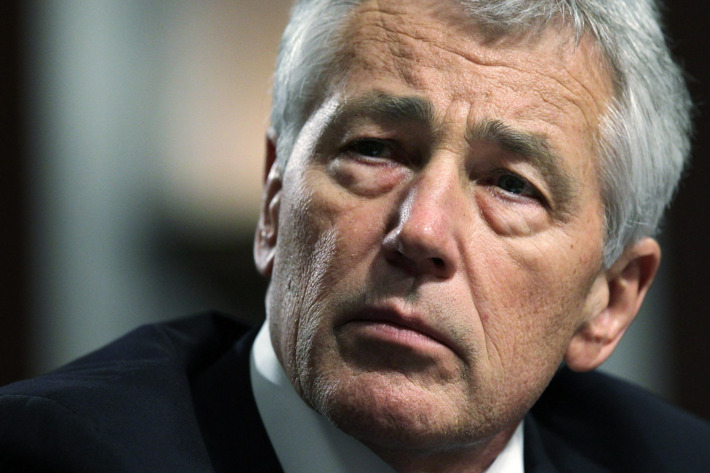
\includegraphics[width=0.3\linewidth, keepaspectratio]{123apictures-sad-faces-162434-9053652}
		\begin{tabular}
					{|c|c|}\hline
					Emocije & [neut, angr, cont, disg, fear, hppy, sadd, surp]\\
					Istinita emocija & [0.00, 0.00, 0.00, 0.00, 0.00, 0.00, 1.00, 0.00]\\
					Predviđena emocija	& [0.45, 0.00, 0.00, 0.00, 0.04, 0.00, 0.51, 0.00]\\
					Pogođena dominantna emocija & 1\\
					Preciznost [0-1] & 0.51\\
					\hline
		\end{tabular}
\end{figure}

Model je ispravno predvidio dominantnu emociju prikazanu na slici iako je rezultat predviđanja zapravo smisleniji od istinite emocije. Istinita emocija ukazuje na potpunu tugu iako to nije slučaj. Crte na licu povlače lice prema dolje, oči sadržavaju tužan pogled a sjena na ustima dodatno naglašava usnice usmjerene prema dolje.

\begin{figure}[H]
\centering
		
\includegraphics[width=0.3\linewidth, keepaspectratio]{255ajose-mourinho.png}
		\begin{tabular}
					{|c|c|}\hline
					Emocije & [neut, angr, cont, disg, fear, hppy, sadd, surp]\\
					Istinita emocija & [0.00, 0.00, 0.00, 1.00, 0.00, 0.00, 0.00, 0.00]]\\
					Predviđena emocija	& [0.01, 0.07, 0.00, 0.92, 0.00, 0.00, 0.00, 0.00]\\
					Pogođena dominantna emocija & 1\\
					Preciznost [0-1] & 0.92\\
					\hline
		\end{tabular}
\end{figure}

Podatkovni skup Google bio je puno zahtjevniji za obradu nego CK+ podatkovni skup. Već u početku ima nesavršenu oznaku emocija za odgovarajuću sliku što direktno utječe na uspješnost treniranja modela. Apstraktnije neviđene slike unutar skupa same su po sebi različite što se tiče osnovnih značajki slika. Za ispravnije korištenje slika preuzetih sa Google-a bilo bi potrebno detaljno proći kroz sve preuzete slike i eventualno promijeniti istinitu emociju za problematične slike. Ukupna točnost nad podatkovnim skupom Google iznosi 51\%. Problematična emocija bila je prezir koji je bio i najmanje zastupljen u Google podatkovnom skupu. Nedostatak slika za treniranje nije dopustio modelu da točnije nauči predviđati emociju prezira.

\begin{figure}[H]
\centering
		\begin{tabular}
					{|c|c|}\hline
					Emocije & [neut, angr, cont, disg, fear, hppy, sadd, surp]\\
					Preciznost emocija& [0.43, 0.63, 0.23, 0.48, 0.42, 0.65, 0.49, 0.55]\\
					Ukupna točnost predviđanja & 51\%\\
					\hline
		\end{tabular}
		\caption{Rezultati testiranja Google podatkovnog skupa}
\end{figure}


\subsection{Rezultati za oba podatkovna skupa}

Zbrojena točnost nad oba podatkovna skupa iznosi 71\%. Oba su podatkovna skupa bila korištena prilikom treniranja da se poveća mogućnost predviđanja modela za neviđene slike ne slične onima iz korištenih podatkovnih skupova. Konfuzijska matrica prikazana na slici \ref{pic:matrix_full} prikazuje odnose emocija ovisno o emociji koja je bila ispravna s obzirom na previđenu emociju. Drugim riječima, slika ukazuje koju je emociju model predvidio s obzirom na istinitu emociju. Zbroj svakog stupca je 1. Redci prikazuju emocije koje su istinite a stupci predstavljaju emociju koju je model predvidio. Primjerice, za istinitu emociju iznenađenja \engl{surprise} model je 20\% (0.2) previdio emociju gađenja. Dijagonala matrice prikazuje ispravno previđene emocije.

Miješanje neutralne emocije sa ostalim primarno proizlazi iz CK+ podatkovnog skupa gdje neutralna emocija ima značajniji utjecaj s obzirom na Google podatkovni skup. Prezir \engl{contempt} često je krivo previđen kao najblaža emocija od spomenutih osam koja je i brojčano najmanje zastupljena prilikom treniranja. Strah \engl{fear} je najčešće pogođena emocija koja je na slikama za model lako prepoznatljiva prema široko otvorenim ustima i očima. Ljutnja \engl{anger} također je laka za predvidjeti s obzirom na ostale emocije zbog često stisnutih zubiju i ukošenih obrva. Konfuzijska matrica govori više o samoj domeni predviđanja emocija i koje emocije dijele sličnosti po pitanju izraza ljudskog lica. Uvidom u problematične emocije moguće je nadograditi podatkovni skup za slikama i oznakama slika koje omogućiti modelu da raspoznaje značajke čija prisutnost nije bila dovoljna prilikom treniranja. 

\begin{figure}[H]
\centering
		\begin{tabular}
					{|c|c|}\hline
					Emocije & [neut, angr, cont, disg, fear, hppy, sadd, surp]\\
					Preciznost emocija& [0.88, 0.72, 0.48, 0.65, 0.59, 0.76, 0.53, 0.67]\\
					Ukupna točnost predviđanja & 71\%\\
					\hline
		\end{tabular}
		\caption{Rezultati testiranja nad oba podatkovna skupa}
\end{figure}


\begin{figure}[H]
\centering
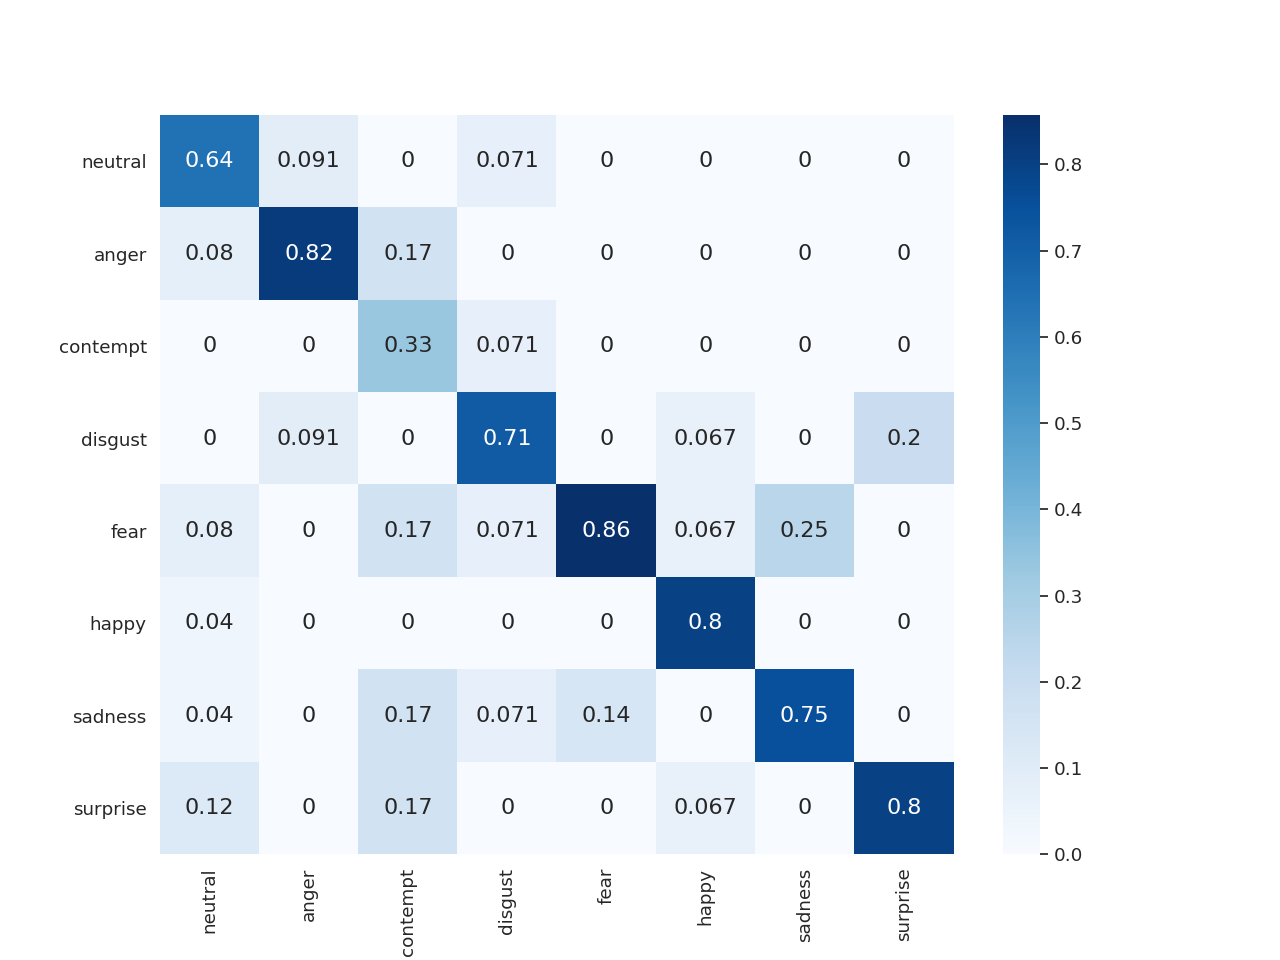
\includegraphics[width=\linewidth, height=0.3\paperheight, keepaspectratio]{matrix_full.png}
\caption{Konfuzijska matrica za oba podatkovna skupa}
\label{pic:matrix_full}
\end{figure}




\chapter{Zaključak}
Korištenjem dva podatkovna skupa i alata PyTorch istrenirani model može do određene točnosti predviđati koju emociju izražava slika ljudskog lica. Uvođenjem dodatnog ručno generiranog Google podatkovnog skupa poboljšana je apstrakcija prepoznavanja emocija koja dopušta modelu da bolje predviđa emocije sa neviđenih slika lica koje nisu slične slikama iz podatkovnog skupa CK+. Točnost predviđanja emocija može biti poboljšana uvođenjem većeg i apstraktnijeg podatkovnog skupa koji sadrži raznolike slike ljudskih lica. 

\bibliography{literatura}
\bibliographystyle{fer}



\begin{sazetak}
Ljudske emocije temeljni dio svih mogućih ljudskih radnji. Treniranjem modela pomoću strojnog učenja koji može klasificirati emocije na temelju slika ljudskih lica otvaraju se mogućnosti za objektivno analiziranje ljudskog ponašanja i razmišljanja u široko primjenjivim situacijama. Uz dva podatkovna skupa ljudskih lica, ResNet50 mrežu i prijenosnim učenjem ponovno istrenirani model može klasificirati neviđene slike ljudskog lica sa 71\% točnosti.

\kljucnerijeci{strojno učenje, duboko učenje, rezidualne neuronske mreže, emocija, lice}
\end{sazetak}

% TODO: Navedite naslov na engleskom jeziku.
\engtitle{Recognizing Emotions From Facial Expressions Using Machine Learning}
\begin{abstract}
Human emotions are the base of all human activities. Training a model 
by using a machine learning method which can later classify emotions given an image of a human facial expression opens up a possibility for an objective analysis of human behaviour and thought process in diverse situations. With two datasets containing images of human facial expressions, ResNet50 network and transferred learning method the trained model can classify emotions given an unseen image of human facial expression with an accuracy of 71\%

\keywords{machine learning, deep learning, residual neural network, emotion, face}
\end{abstract}

\end{document}
